\documentclass{article}
\usepackage[utf8]{inputenc}

\usepackage{biblatex}
\usepackage{amsmath,amsthm, amssymb}
\usepackage[margin=3cm]{geometry}
\usepackage{mathtools}
\usepackage{dsfont}
\usepackage{xcolor}
\usepackage{algorithm,algpseudocode}
\usepackage{todonotes}
\usepackage{nicefrac}
\usepackage{mathrsfs}
\usepackage{tikz}
\usepackage{thm-restate}
\usepackage{hyperref}

\usepackage{etoc}

%%%%%%%%    THEOREM DEFINITIONS AND RESTATABLE
% \newcounter{claim}
% \setcounter{claim}{0}
\newtheorem{theorem}{Theorem}
\newtheorem{lemma}[theorem]{Lemma}
\newtheorem{corollary}[theorem]{Corollary}
\newtheorem{claim}{Claim}
\newtheorem{dependency}{Dependency}
\newtheorem{definition}{Definition}

\newcommand{\matt}[1]{\todo[color=red!50, prepend, caption={Matt}, tickmarkheight=0.25cm]{#1}}
\newcommand{\inlinetodo}[1]{\textcolor{red}{{\Large TODO:} #1}}

\newcommand{\on}{\text{on}}
\newcommand{\off}{\text{off}}

%%%%%%%%    NOTATION DEFINITIONS FOR EASIER WRITING
\newcommand{\ket}[1]{|#1\rangle}
\newcommand{\bra}[1]{\langle #1|}
\newcommand{\braket}[2]{\langle #1|#2\rangle}
\newcommand{\ketbra}[2]{| #1\rangle\! \langle #2|}
\newcommand{\parens}[1]{\left( #1 \right)}
\newcommand{\brackets}[1]{\left[ #1 \right]}
\newcommand{\abs}[1]{\left| #1 \right|}
\newcommand{\norm}[1]{\left| \left| #1 \right| \right|}
\newcommand{\diamondnorm}[1]{\left| \left| #1 \right| \right|_\diamond}
\newcommand{\anglebrackets}[1]{\left< #1 \right>}
\newcommand{\overlap}[2]{\anglebrackets{#1 , #2 }}
\newcommand{\set}[1]{\left\{ #1 \right\}}
\newcommand{\ceil}[1]{\left\lceil #1 \right\rceil}
\newcommand{\openone}{\mathds{1}}
\newcommand{\expect}[1]{\mathbb{E}\brackets{#1}}
\newcommand{\variance}[1]{\textit{Var} \brackets{ #1 }}
\newcommand{\prob}[1]{\text{Pr}\left[ #1 \right]}
\newcommand{\bigo}[1]{O\left( #1 \right)}
\newcommand{\bigotilde}[1]{\widetilde{O} \left( #1 \right)}
\newcommand{\ts}{\textsuperscript}

\DeclareMathOperator{\Tr}{Tr}
\newcommand{\trace}[1]{\Tr \brackets{ #1 }}
\newcommand{\partrace}[2]{\Tr_{#1} \brackets{ #2 }}
\newcommand{\complex}{\mathbb{C}}

%%%%% COMMONLY USED OBJECTS
\newcommand{\hilb}{\mathcal{H}}
\newcommand{\partfun}{\mathcal{Z}}
\newcommand{\identity}{\mathds{1}}
\newcommand{\gue}{\rm GUE}
\DeclareMathOperator{\sinc}{sinc}
\DeclareMathOperator{\hermMathOp}{Herm}
\DeclareMathOperator{\im}{Im}
\DeclareMathOperator{\diag}{diag}
\newcommand{\herm}[1]{\hermMathOp\parens{#1}}


\title{Quantum Thermal State Preparation via Repeated Interactions}
\author{Matthew Hagan, Nathan Wiebe}
\date{May 2022}

\begin{document}

\maketitle
% \abstract{The repeated interactions framework is a theoretical method of thermalization for open quantum systems that proposes systems reach thermal equilibrium by interacting with small, single qubit, ``environments" that are in themselves in thermal equilibrium. The mental model is many photons bombarding a sample, each interacting for some time only to be replaced by a fresh photon after some interaction time. We study this model through the lens of quantum algorithm design by modeling the interaction hamiltonian with a random ensemble that resembles the GUE distribution and studying the dynamics in a weak-coupling or short-time regime. Our main insight is that the dynamics of the repeated interactions channel acting on a quantum state is controllably close to a Markov chain over the eigenstates of the system Hamiltonian. The fixed points and spectral gap of this Markov chain are dictated by the eigenvalue gap of the environment Hamiltonians. One crucial benefit of this Markov chain is that if configured properly the fixed point is a thermal state of the system automatically and bypasses the need for filtration techniques of Metropolis-Hastings style algorithms. As we further only need quantum simulation as a sub-routine this algorithm should be viewed as the quantum generalization of Hamiltonian Monte Carlo techniques. We provide detailed analysis for an arbitrary single qubit system, including analytic runtime bounds for both knowledge of the eigenvalue gap and probabilistic analysis based on a distribution of the eigenvalue gap. We also analyze a truncated Harmonic Oscillator and show that the thermal state is a fixed point and provide numeric bounds on the Markov relaxation time. For generic systems we show that in the zero-temperature limit the ground state is a fixed point. We provide numeric results for the single qubit, harmonic oscillator, and hydrogen chains. The harmonic oscillator numerics display a Mpemba phenomenon, when starting from the infinite temperature aka maximally mixed state, where lower temperature states require less interactions and interaction time to thermalize than some intermediate temperature states.}

% \begin{center}
%     \textbf{Abstract 2.0}
% \end{center}
% The preparation of good initial states for the simulation of quantum systems on digital quantum devices is an active area of research, as many of the existing algorithms have significant drawbacks. In this paper we propose a novel algorithm for the preparation of thermal states by combining ideas from the repeated interactions or collisional model of thermalization from open quantum systems literature and Hamiltonian Monte Carlo techniques from machine learning. The algorithm consists of preparing a single environment qubit in a thermal state at inverse temperature $\beta$ and a user specified eigenvalue gap $\gamma$ and then simulating the time dynamics of the system of interest with a random interaction Hamiltonian to couple the ancilla qubit to the system. The dynamics of the channel in the weak-coupling/long-time or strong-coupling/short-time regime reduce to a Markov chain over the eigenstates of the system Hamiltonian. This Markov chain has the thermal state $e^{-\beta H} / \partfun$ as a fixed point, bypassing the need for complicated sample rejection techniques (such as Marriot-Watrous rewinding) present in quantum analogs of Metropolis-Hastings style algorithms. We study the performance of this algorithm in detail for arbitrary single qubit Hamiltonians and the truncated Harmonic oscillator, with numeric evidence showcasing a Quantum Mpemba effect in the Harmonic oscillator. We further provide analytic evidence that the thermal state is the fixed point if one can sample eigenvalue differences exactly for any Hamiltonian and we show numeric evidence that this requirement is not restrictive for small hydrogen chain systems. 

% \begin{center}
%     \textbf{Abstract 3.0}
% \end{center}
\abstract{
The simulation of quantum systems remains the most promising application for future digital quantum computers after decades of theoretic exploration. Most research has gone into developing better algorithms for simulating the time dynamics, with initial state preparation posing the most challenging open problem. In this paper we propose a novel quantum algorithm for the preparation of quantum thermal states $e^{-\beta H} / \partfun$ based on a synthesis of ideas from the Repeated Interactions framework in the open quantum systems literature and Hamiltonian Monte Carlo techniques from machine learning. Our algorithm works by preparing the ancilla in a thermal state, coupling the ancilla and system with a random matrix with Haar distributed eigenvectors and I.I.D Gaussian eigenvalues, and then simulating the time dynamics of the now coupled system-ancilla before removing the ancilla. We show that the quantum dynamics of this channel is arbitrarily close to a classical Markov chain over the eigenstates of $H$ which, when tuned properly, has the thermal state as it's fixed point. This Markov chain crucially avoids any complicated rejection or unwinding steps present in most previous quantum Metropolis-Hastings inspired algorithms, which significantly simplifies the implementation. The runtime of our algorithm scales like the inverse of the spectral gap of the resulting Markov chain, which is to be expected. We provide detailed analysis for the harmonic oscillator, which displays a surprisingly complicated Mpemba phenomenon, and we show that low temperature thermal states of small hydrogen chains can be prepared by choosing random energy gaps for the ancilla hamiltonian. 
}
\tableofcontents

%%%%%%%%%%%%%%%%%%%%%%%%%%%%%%%%%%%%%%%%%%%%%%%%%%%%%%%%%%%%%%%%%%%%%%%%%%%%%%%%%%%%%%%%%%%%%%%%%%%%%%%%%%%%%%%%%%%%%%%%%%%%%%%%%%%%%%%%%%%%%%%%
%%%%%%%%%%%%%%%%%%%%%%%%%%%%%%%%%%%%%%%%%%%%%%%%%%%%%%%%%%%%%%%%%%%%%%%%%%%%%%%%%%%%%%%%%%%%%%%%%%%%%%%%%%%%%%%%%%%%%%%%%%%%%%%%%%%%%%%%%%%%%%%%
%%%%%%%%%%%%%%%%%%%%%%%%%%%%%%%%%%%%%%%%%%%%%%%%%%%%%%%%%%%%%%%%%%%%%%%%%%%%%%%%%%%%%%%%%%%%%%%%%%%%%%%%%%%%%%%%%%%%%%%%%%%%%%%%%%%%%%%%%%%%%%%%
\section{Introduction}
Going to leave this blank for now. \cite{shiraishi_undecidability_2021}

%%%%%%%%%%%%%%%%%%%%%%%%%%%%%%%%%%%%%%%%%%%%%%%%%%%%%%%%%%%%%%%%%%%%%%%%%%%%%%%%%%%%%%%%%%%%%%%%%%%%%%%%%%%%%%%%%%%%%%%%%%%%%%%%%%%%%%%%%%%%%%%%
%%%%%%%%%%%%%%%%%%%%%%%%%%%%%%%%%%%%%%%%%%%%%%%%%%%%%%%%%%%%%%%%%%%%%%%%%%%%%%%%%%%%%%%%%%%%%%%%%%%%%%%%%%%%%%%%%%%%%%%%%%%%%%%%%%%%%%%%%%%%%%%%
%%%%%%%%%%%%%%%%%%%%%%%%%%%%%%%%%%%%%%%%%%%%%%%%%%%%%%%%%%%%%%%%%%%%%%%%%%%%%%%%%%%%%%%%%%%%%%%%%%%%%%%%%%%%%%%%%%%%%%%%%%%%%%%%%%%%%%%%%%%%%%%%
\section{Preliminaries}
We denote the Hilbert space of the system as $\hilb_{S}$ and the environment as $\hilb_{E}$, with the Hamiltonians governing each as $H_{S}$ and $H_{E}$. We will assume without loss of generality that the system's Hilbert space can be encoded with $n$ qubits, giving $\dim_S = 2^{n}$, and the environment's Hilbert space can be encoded with $m$ qubits giving $\dim_E = 2^{m}$. The Hamiltonian for the joint system on $\hilb_{S} \otimes \hilb_{E}$ is then $H = H_{S} \otimes \identity + \identity \otimes H_{E}$. The Hilbert space of the combined system and environment is of dimension $\dim = \dim_E \cdot \dim_S = 2^{n + m}$. 

We will primarily work in the eigenbasis for each Hamiltonian:
\begin{equation}
    H_{S} = \sum_{i = 0}^{2^n - 1} \lambda_S(i) \ketbra{s_i}{s_i} ~,~ H_{E} = \sum_{j=0}^{2^m - 1} \lambda_E(j) \ketbra{e_j}{e_j} ~,~ H = \sum_{i=0}^{2^n - 1} \sum_{j=0}^{2^m - 1} \lambda(i,j) (\ket{s_i} \otimes \ket{e_j})(\bra{s_i} \otimes \bra{e_j}),
\end{equation}
for convenience we will denote the tensor product of eigenvectors simply by their indices $\ket{i,j} \coloneqq \ket{s_i} \otimes \ket{e_j}$. For convenience we define $\lambda(i,j) \coloneqq \lambda_S(i) + \lambda_E(j)$. We also make use of the following notation for the energy differences of the system-environment Hamiltonian
$$\Delta(i,j|k,l) \coloneqq \lambda(i,j) - \lambda(k,l),$$
and will use $\Delta_S(i,j) \coloneqq \lambda_S(i) - \lambda_S(j)$ for just the system differences. We use the notation $\delta(i,j|k,l)$ to denote the product of Kronecker delta functions $\delta(i,j|k,l) = \delta_{i,k} \delta_{j,l}$.

For input states we will typically assume thermal states of the form $\rho_S(\beta) = \frac{e^{-\beta H_S}}{\partfun_S}$, where $\partfun_S = \trace{e^{-\beta H_S}}$, where the inverse temperature $\beta$ of the partition function will typically be assumed but written explicitly if need be. We will assume environment states of the form $\rho_E(\beta) = \frac{e^{-\beta H_E}}{\partfun_E}$.


Overall one application of our channel is represented as
\begin{equation}
    \Phi(\rho ; \alpha, \beta_E, t) :=  \partrace{\hilb_E}{\int e^{+i(H + \alpha G)t} \rho \otimes \rho_E(\beta_E) e^{-i(H + \alpha G) t} dG},
\end{equation}
and we will typically let the parameters $\alpha, \beta_E,$ and $t$ for the channel be implicit. It will prove convenient to study the time evolution of a fixed interaction as a map from the total system-environment Hilbert space to itself. We denote this channel for a fixed interaction $G$ as
\begin{equation}
    \Phi_G(\rho_S \otimes \rho_E(\beta_E) := e^{+i (H+ \alpha G) t} \rho_S \otimes \rho_E(\beta_E) e^{-i (H + \alpha G) t}. \label{eq:phi_g_definition}
\end{equation}
Clearly then $\Phi(\rho_S) = \partrace{\hilb_E}{\int \Phi_G (\rho_S \otimes \rho_E) dG}$. We use $G$ to denote the randomized interaction term, where $G = U_G D U_G^\dagger$. The measure we choose for the eigenbasis of $G$ is $U_G \sim Haar$ and the eigenvalues are i.i.d with mean 0 and variance $1$.  This gives the overall interaction measure as the decomposition $\int dG = \int \int dD ~ dU_G$. The interaction strength of $G$ will be controlled through the coupling coefficient $\alpha$.

\begin{restatable}{lemma}{haar_two_moment} \label{lem:haar_two_moment}
    Let $\int (\cdot) dU$ denote the average distributed according to the Haar measure over $\dim$-dimensional unitary matrices $U$. Then for $\ket{i_1},\ket{i_2},\ldots,\ket{k_2}$ drawn from an orthonormal basis
    \begin{align}
        &\int \bra{i_1} U \ket{j_1} \bra{i_2} U \ket{j_2} \bra{k_1} U^\dagger \ket{l_1} ~ \bra{k_2} U^\dagger \ket{l_2} dU \nonumber \\
        &= ~\frac{1}{\dim^2 - 1} \parens{\delta_{i_1, l_1} \delta_{j_1, k_1} \delta_{i_2, l_2} \delta_{j_2, k_2} + \delta_{i_1, l_2} \delta_{j_1, k_2} \delta_{i_2, l_1} \delta_{j_2, k_1}} \nonumber \\
        &\quad - \frac{1}{\dim(\dim^2 - 1)} \parens{\delta_{i_1, l_2} \delta_{j_1, k_1} \delta_{i_2, l_1} \delta_{j_2, k_2} + \delta_{i_1, l_1} \delta_{j_1, k_2} \delta_{i_2, l_2} \delta_{j_2, k_1}}. \label{eq:haar_two_moment_integral}
    \end{align}
\end{restatable}


\section{Taylor's Series for $\Phi$} \label{sec:taylor_series_phi}

The easiest way for us to understand the thermalizing channel $\Phi$ is through a Taylor's series with respect to the coupling constant $\alpha$, which will turn out to give us a series in terms of $\alpha t$ instead. This can be thought of as the weak interaction regime, which is extensively studied in open quantum systems. This section provides results about the first and second order terms in the Taylor's Series for $\Phi$ and we give an upper bound on the norm of the remainder term $R_{\Phi}$. As many of the proofs for the statements in this section tend to be rather technical and do not lend themselves to much insight they can be found in the appendix. 

$\Phi$ can be written with the mean-value version of Taylor's theorem as:
\begin{equation}
    \Phi(\rho_S; \alpha) = \Phi(\rho_S; \alpha = 0) + \alpha \frac{\partial}{\partial \alpha} \Phi(\rho_S; \alpha) \bigg|_{\alpha = 0} + \frac{\alpha^2}{2!} \frac{\partial^2}{\partial \alpha^2} \Phi(\rho_S; \alpha) \bigg|_{\alpha = 0} + R_{\Phi}(\rho_S, \alpha_{\star}).
\end{equation}
We will denote the second order approximation as
\begin{equation}
    \Phi^{(2)}(\rho_S) \coloneqq \Phi(\rho_S) - R_{\Phi}(\rho_S, \alpha_\star) = \Phi(\rho_S;\alpha= 0) + \frac{\partial}{\partial \alpha} \Phi(\rho_S, \alpha) \bigg|_{\alpha = 0} + \frac{1}{2!} \frac{\partial^2}{\partial \alpha^2} \Phi(\rho_S, \alpha) \bigg|_{\alpha = 0}. \label{def:second_order_approx}
\end{equation}
We will also find it helpful to denote each of the terms as
\begin{equation}
    T^{(k)}(X, \alpha) \coloneqq \frac{\alpha^k}{k!} \frac{\partial^k}{\partial \alpha^k} \Phi(X, \alpha)\bigg|_{\alpha = 0}.\label{def:taylor_series_terms}
\end{equation}
If we were to write out the channel $\Phi$ as a Taylor's Series it would be $\Phi(\rho_S) = \sum_{k = 0}^{\infty} T^{(k)}(\rho_S)$.

We now go through and compute the correction terms $T^{(0)}$, $T^{(1)}$, and $\mathcal{T}^{(2)}$. The first one is nearly trivial
\begin{lemma}
    The zeroth order correction $T^{(0)}$ to the thermalizing channel $\Phi$ is the Heisenberg evolved input 
    \begin{equation}
        T^{(0)}(\rho_S) = e^{i H_S t} \rho_S e^{-i H_S t},
    \end{equation}
    where this expression holds for all matrix inputs and not just density operators.
\end{lemma}
\begin{proof}
This is a straightforward computation after plugging in the definitions
    \begin{align}
        T^{(0)}(\rho_S) &= \partrace{\hilb_E}{\int e^{i(H + 0 G)t} \rho_S \otimes \rho_E(\beta_E) e^{-i(H + 0 G)t} dG } \\
        &= \partrace{\hilb_E}{e^{i (H_S \otimes \identity + \identity \otimes H_E)t} \rho_S \otimes \rho_E(\beta_E) e^{-i (H_S \otimes \identity + \identity \otimes H_E)t}} \\
        &= e^{i H_S t} \rho_S e^{-i H_S t}.
    \end{align}
\end{proof}
It will prove useful that this result holds even if we extend the $\rho_S$ input to an arbitrary matrix input, as nowhere in the proof did we rely on the properties of density matrices. This will be necessary in arguing that coherences, or off-diagonal matrix elements in a density matrix, do not accumulate with repeated uses of our channel.

The next order correction shows that to $O(\alpha)$ the effects of the environment on the system are zero. This shows that higher order corrections are necessary to compute nontrivial environmental effects. We leave this proof in this section to give the reader a taste for how these arguments work in the higher order calculations. This proof in particular solely relies on the randomly chosen eigenvalues of the interaction to be mean 0.
\begin{lemma}
   The first order correction $T^{(1)}$ to the thermalizing channel $\Phi$, with randomized interactions $G = U_G D U_G^\dagger $ such that the average of each eigenvalue satisfies $\mathbb{E}[d_{i,i}] = 0$, is zero:
   \begin{equation}
        T^{(1)}(\rho_S) = 0.
   \end{equation}
\end{lemma}
\begin{proof}
    We start by using linearity of derivatives, integration, and partial trace to compute the action of the $\alpha$ derivative on $\Phi_G$ as
    \begin{align}
        \frac{\partial}{\partial \alpha} \Phi(\rho_S) \bigg|_{\alpha = 0} &= \frac{\partial}{\partial \alpha} \partrace{\mathcal{H}_E}{\int \Phi_G(\rho_S) dG} \bigg|_{\alpha = 0} \\
         &= \partrace{\mathcal{H}_E}{\int \frac{\partial}{\partial \alpha} \Phi_G(\rho_S) dG \bigg|_{\alpha = 0} } .
    \end{align}
    Now we use the expression for $\Phi_G$ in Eq. \eqref{eq:phi_g_definition} to compute the derivatives, and we denote the total system-environment state as $\rho = \rho_S \otimes \rho_E(\beta_E)$,
    \begin{align}
        \frac{\partial}{\partial \alpha} \Phi_G (\rho_S) &= \parens{\frac{\partial}{\partial \alpha} e^{+ i (H + \alpha G)t}} \rho e^{-i (H + \alpha G) t} + e^{+i (H + \alpha G)t} \rho \parens{\frac{\partial}{\partial \alpha} e^{- i (H + \alpha G)t}} \\
        &= \parens{\int_{0}^{1} e^{i s (H+\alpha G)t} (i t G) e^{i (1-s) (H+\alpha G)t} ds} \rho e^{-i(H+\alpha G)t} \nonumber \\
    &~ ~+ e^{i(H+\alpha G)t} \rho \parens{\int_{0}^1 e^{-i s (H+\alpha G) t} (- i t G) e^{-i (1-s) (H+\alpha G)t} ds}. \label{eq:first_order_alpha_derivative}
    \end{align}
    We can further simplify this by bringing in the evaluation of $\alpha = 0$ through the partial trace and integration, as they are uniformly convergent over $\alpha$ (is that the correct notion that allows us to switch orders?)
    \begin{align}
        \frac{\partial}{\partial \alpha} \Phi_G(\rho_S) \bigg|_{\alpha = 0} &= i t \int_0^1 e^{i s H t} G e^{-i s H t} ds e^{i H t} \rho e^{-i H t} - i t e^{+i H t} \rho \int_0^1 e^{-is H t} G e^{-i(1-s) Ht} ds \\
        &= i t \parens{\int_0^1 G(s t) ds} \rho(t) - it \rho(t) \parens{\int_0^1 G(s t) ds} \\
        &= i t \int_0^1 [G(s t), \rho(t)] ds,
    \end{align}
    where we have used the Heisenberg picture $\rho(t) = e^{i H t} \rho e^{-i H t}$ to simplify the notation.

    This expression is now amenable to computing the correction to the total channel. We do so by performing the integration over the randomized interactions. We take advantage of the structure of our interaction measure, that is $G = U_G D U_G^\dagger$ and $dG = dU_G dD$, which allows us to write
    \begin{align}
        \int \frac{\partial}{\partial \alpha} \Phi_G(\rho_S) \bigg|_{\alpha = 0} dG &= it \int \int_0^1 \left[ e^{i H s t} G e^{-i H s t}, \rho(t) \right] ds ~dG \\
        &= it \int_0^1 \left[ e^{i H s t} \parens{\int \int U_G D U_G^\dagger ~dU_G ~ dD} e^{-i H s t}, \rho(t)  \right] ds \\
        &= i t \int_0^1 \left[ e^{i H s t} \parens{\int U_G \parens{\int D ~ dD} ~ U_G^\dagger dU_G } e^{-i H s t}, \rho(t) \right] ds \\
        &= 0.
    \end{align}
    This last step relies on the use of random eigenvalues with mean 0, implying $\int D ~dD = 0$, which yields the statement.
\end{proof}

Now we move on to calculating the second order correction $\mathcal{T}$. This is a significantly more tedious computation, so we move the proof of this result to the appendices. First we compute the ``pre-trace" matrix elements of the second order correction $\mathcal{T}$ but only for diagonal input matrices. It will turn out that $\mathcal{T}$ does not introduce any new coherences to the quantum state, which will be shown later. For now, the raw output of the channel is given in the following lemma.

\begin{restatable}[Second Order Correction]{lemma}{secondOrderChannelHaar} \label{lem:big_one}
    Given a system Hamiltonian $H_{S}$, an environment Hamiltonian $H_{E}$, a simulation time $t$, and coupling coefficient $\alpha$, let $\Phi_G : \hilb_S \otimes \hilb_E \to \hilb_S \otimes \hilb_E$ denote the fixed interaction channel 
    \begin{equation}
        \Phi_G(\rho) = e^{+i (H + \alpha G)t} \rho e^{-i (H + \alpha G)t},
    \end{equation}
    where $H = H_S \otimes \identity + \identity \otimes H_E$. Let $\chi$ denote the following coherence prefactor
$$ \chi(i,j) \coloneqq \sum_{a,b: \Delta(i,j,|a,b) \neq 0} \frac{1 - i \Delta(i,j|a,b)t - e^{-i \Delta(i,j|a,b) t}}{\Delta(i,j|a,b)^2} $$
and $\eta(i,j) \coloneqq \sum_{a, b} \mathbf{I}[\lambda(i,j) = \lambda(a, b)]$ denote the degeneracy of the $(i,j)$ eigenvalue. Then the $\bigo{\alpha^2}$ term of $\Phi_G$ is given by the following:
 \begin{align}
     \int \frac{\alpha^2 }{2}\frac{\partial^2}{\partial \alpha^2} \Phi_G(\ketbra{i,j}{k,l})\bigg|_{\alpha = 0} dG &= -\frac{\alpha^2  e^{i \Delta(i,j|k,l) t}}{\dim + 1} \bigg(\chi(i,j) + \chi(k,l)^*  + \frac{t^2}{2}(\eta(i,j) + \eta(k,l)) \bigg) \ketbra{i,j}{k,l} \nonumber \\
    &~ + \mathbf{I}[(i,j) = (k,l)]  \frac{\alpha^2 t^2}{\dim+1} \sum_{a,b} \sinc^2 \left( \frac{\Delta(i,j|a,b)t}{2} \right) \ketbra{a,b}{a,b}  \label{eq:el_gigante}
 \end{align}
\end{restatable}
The proof of this is given in Appendix \ref{sec:haar_integral_appendix}. 

These can be seen from Lemma \ref{lem:big_one}.

\begin{lemma} \label{lem:t_2_both}
    The diagonal elements in the pre-trace second order correction are given as
    \begin{align}
        &\int \bra{i', j'} \mathcal{T}_G \left( \ketbra{i, j}{i, j} \right) \ket{i', j'} ~dG \\
        &= \begin{cases}
            - \frac{\alpha^2 t^2 }{\dim + 1} \sum_{(a,b) \neq (i, j)} \sinc^2(\Delta(a,b|i,j) t / 2) & (i,j) = (i', j') \\
    \frac{\alpha^2 t^2 }{\dim + 1} \sinc^2(\Delta(i,j | i', j') t /2) & (i, j) \neq (i', j'),
        \end{cases} \label{eq:second_order_transitions_final_final}
    \end{align}
    where we use the fact that $\lim_{x \to 0} \sinc(x) = 1$ to compute the degenerate contributions (when $\Delta(i, j | i', j') = 0$)
\end{lemma}
However, if we want to compute the effects of the channel on a given input, we have to perform the partial trace over the environment, which clearly depends on initial state of the environment we choose. To proceed, we choose a simple two-level environment $H_E = \begin{bmatrix}
    0 & 0 \\ 0 & \gamma
\end{bmatrix}$, where the eigenvectors $\ket{0}$ and $\ket{1}$ have eigenvalues 0 and $\gamma$ respectively. Here, and throughout the rest of the paper, $\gamma$ should be thought of as a user defined parameter that can be adjusted, or chosen probablistically, throughout the cooling procedure. We use a thermal input state $\rho_E(\beta_E)$, as defined in the preliminaries. 

\begin{lemma} \label{lem:on_and_off_resonance}
    The effects of the second order term of our channel into those that significantly contribute to the result and those that can be suppressed, in symbols $\mathcal{T}(\rho) = \mathcal{T}_{\on}(\rho) + \mathcal{T}_{\off}(\rho)$. We can compute these using 

\begin{align}
    \mathcal{T}(X) &= \mathcal{T}_{\on}(X) + \mathcal{T}_{\off}(X) \\
    \bra{j}\mathcal{T}_{\on}(\ketbra{i}{i}) \ket{j} &= \begin{cases}
        \widetilde{\alpha}^2 \frac{e^{-\beta_E \gamma}}{1 + e^{-\beta_E \gamma}} \sinc^2\left(\frac{(\Delta_S(i,j) + \gamma)t}{2}\right) & i < j \text{ and } |\Delta_S(i,j) - \gamma| \le \Delta_{\min} \\
        \widetilde{\alpha}^2 \frac{1}{1 + e^{-\beta_E \gamma}} \sinc^2\left(\frac{(\Delta_S(i,j) - \gamma)t}{2}\right) & i > j \text{ and } |\Delta_S(i,j) - \gamma| \le \Delta_{\min} \\
        - \sum_{k \neq i} \bra{k} \mathcal{T}_{\on}(\ketbra{i}{i})\ket{k} & i = j
    \end{cases} \\
    \bra{j}\mathcal{T}_{\off}(\ketbra{i}{i}) \ket{j} &= \begin{cases}
        \widetilde{\alpha}^2 \left( \sinc^2(\Delta_S(i,j) t/2) + \frac{1}{1 + e^{-\beta_E \gamma}} \sinc^2\left( \frac{(\Delta_S(i,j) - \gamma) t}{2}\right) \right) & i < j \\
        \widetilde{\alpha}^2 \left( \sinc^2(\Delta_S(i,j) t/2) + \frac{e^{-\beta_E \gamma}}{1 + e^{-\beta_E \gamma}} \sinc^2\left( \frac{(\Delta_S(i,j) + \gamma) t}{2}\right) \right) & i > j \\
        -\widetilde{\alpha}^2 \sum_{k \neq i}\sinc^2\left(\frac{\Delta_S(k, i)t}{2}\right) - \widetilde{\alpha}^2\sum_{k \neq i} q(0) \sinc^2 \left(\frac{(\Delta_S(k, i) + \gamma)t}{2} \right) + q(1) \sinc^2 \left(\frac{(\Delta_S(k, i) - \gamma)t}{2} \right) & i = j
    \end{cases},
\end{align}
where we note that all of the off-diagonal contributions require that $|\Delta_S(i,j) - \gamma | \ge \Delta_{\min}$ and $|\Delta_S(k,j) - \gamma | \ge \Delta_{\min}$, we just ran out of space to impose the condition inline. Now what we can do is remove the $\mathcal{T}_{\off}$ terms from the distance upper bound by including them with the remainder term. 
\end{lemma}

\begin{lemma} \label{lem:t_2_system_only}
    The second order correction to the channel $\Phi$ with two level environment as described above, differs if the output state $j$ is less than, equal to, or greater than $i$. For $i < j$, meaning we are transitioning the systme from a lower energy state to a higher energy and the environment is losing energy, we have
    \begin{equation}
        \left| \bra{j}\mathcal{T}^{(2)}(\ketbra{i}{i})\ket{j} - \frac{\alpha^2 t^2}{\dim + 1} \frac{e^{-\beta_E \gamma}}{1 + e^{-\beta_E \gamma}} \sinc^2 \parens{(\Delta_S(i,j) + \gamma) t/ 2} \right| \leq 3 \frac{\alpha^2 t^2}{\dim + 1} \epsilon_{\sinc}.
    \end{equation}
    For $i > j$, meaning we are transitioning the system from a high energy state to a lower energy state, we have
    \begin{equation}
        \left| \bra{j}\mathcal{T}^{(2)}(\ketbra{i}{i})\ket{j} - \frac{\alpha^2 t^2}{\dim + 1} \frac{1}{1 + e^{-\beta_E \gamma}} \sinc^2 \parens{(\Delta_S(i,j) - \gamma) t/ 2} \right| \leq 3 \frac{\alpha^2 t^2}{\dim + 1} \epsilon_{\sinc}.
    \end{equation}
    For $i = j$, where the state does not gain or lose energy, we get contributions from all other system states that are weighted based on the gain or loss of energy and is given by
    \begin{align}
        &\left| \bra{i} \mathcal{T}^{(2)}(\ketbra{i}{i}) \ket{i} + \frac{\alpha^2 t^2}{\dim + 1} \parens{\frac{1}{1 + e^{-\beta_E \gamma}} \sum_{a < i} \sinc^2 ((\Delta_S(a, i) + \gamma) t/ 2) + \frac{e^{-\beta_E \gamma}}{1 + e^{-\beta_E \gamma}} \sum_{a > i} \sinc^2((\Delta_S(a, i) - \gamma)t/ 2)} \right| \nonumber \\
        &\leq 4 \dim_S \frac{\alpha^2 t^2}{\dim + 1} \epsilon_{\sinc},
    \end{align}
    where we point out the difference in sign for the $i = j$ terms and the $i \neq j $ terms.
\end{lemma}
\begin{proof}
    For $i < j$ we use Eq. \eqref{eq:second_order_transitions_final_final} straightforwardly
    \begin{align}
        &\bra{j} \mathcal{T}^{(2)} (\ketbra{i}{i}) \ket{j} \nonumber \\
        &= \frac{1}{1 + e^{-\beta_E \gamma}} \int \parens{\bra{j, 0} \mathcal{T}^{(2)}_G(\ketbra{i,0}{i, 0}) \ket{j, 0} + \bra{j, 1} \mathcal{T}^{(2)}_G (\ketbra{i, 0}{i ,0}) \ket{j, 1} } dG \nonumber \\
        &~+ \frac{e^{-\beta_E \gamma}}{1 + e^{-\beta_E \gamma}} \int \parens{\bra{j, 0} \mathcal{T}^{(2)}_G (\ketbra{i, 1}{i, 1}) \ket{j, 0} + \bra{j, 1} \mathcal{T}^{(2)}_G (\ketbra{i, 1}{i, 1}) \ket{j, 1}} dG \\
        &= \frac{1}{1 + e^{-\beta_E \gamma}} \frac{\alpha^2 t^2}{\dim + 1}\parens{\sinc^2(\Delta_S(i, j) t/ 2) + \sinc^2 (\Delta_S(i, j) - \gamma)t /2} \nonumber \\
        &~+ \frac{e^{-\beta_E \gamma}}{1 + e^{-\beta_E \gamma}} \frac{\alpha^2 t^2 }{\dim + 1} \parens{\sinc^2((\Delta_S(i,j) + \gamma) t/ 2) + \sinc^2(\Delta_S(i,j) t/ 2)} \\
        &= \frac{\alpha^2 t^2}{\dim + 1}\left( \sinc^2(\Delta_S(i,j)t/2) + \frac{1}{1 + e^{-\beta_E \gamma}} \sinc^2((\Delta_S(i,j) - \gamma)t/2) + \frac{e^{-\beta_E \gamma}}{1 + e^{-\beta_E \gamma}} \sinc^2((\Delta_S(i,j) + \gamma)t/2) \right) \label{eq:t_2_intermediate_1}
        \end{align}
    From this expression, we see that since $i < j \implies \Delta_S(i,j) < 0$ we have that $\sinc^2(\Delta_S(i,j)t/2) \leq \epsilon_{\sinc}$ and $\sinc^2((\Delta_S(i,j) - \gamma)t/2) \le \epsilon_{\sinc}$. We can then isolate the only non-negligible term, which leads to the difference
    \begin{align}
        i < j \implies \left| \bra{j}\mathcal{T}^{(2)}(\ketbra{i}{i})\ket{j} - \frac{\alpha^2 t^2}{\dim + 1} \frac{e^{-\beta_E \gamma}}{1 + e^{-\beta_E \gamma}} \sinc^2 \parens{(\Delta_S(i,j) + \gamma) t/ 2} \right| &\le 2 \frac{\alpha^2 t^2}{\dim + 1} \epsilon_{\sinc} \\
        &= \frac{8 \alpha^2}{\Delta_{\min}^2 (\dim + 1)}.
    \end{align}
    For $i > j$ we can start from Eq. \ref{eq:t_2_intermediate_1} and the only difference is that the sinc term with $\Delta_S(i,j) - \gamma$ is the non-negligible term so we get
    \begin{align}
    i > j \implies \left| \bra{j}\mathcal{T}^{(2)}(\ketbra{i}{i})\ket{j} - \frac{\alpha^2 t^2}{\dim + 1} \frac{e^{-\beta_E \gamma}}{1 + e^{-\beta_E \gamma}} \sinc^2 \parens{(\Delta_S(i,j) - \gamma) t/ 2} \right| &\le \frac{8 \alpha^2}{\Delta_{\min}^2 (\dim + 1)}.
        \end{align}
     
    For the $i = j$ calculation we have
    \begin{align}
        \bra{i} \mathcal{T}^{(2)}(\ketbra{i}{i}) \ket{i} &= \frac{1}{1 + e^{-\beta_E \gamma}} \int \bra{i, 0} \mathcal{T}^{(2)}_G (\ketbra{i, 0}{i, 0}) \ket{i, 0} dG + \frac{e^{-\beta_E \gamma}}{1 + e^{-\beta_E \gamma}} \int \bra{i, 0} \mathcal{T}^{(2)}_G (\ketbra{i, 1}{i, 1}) \ket{i, 0} dG \nonumber \\
        &~+ \frac{1}{1 + e^{-\beta_E \gamma}} \int \bra{i, 1} \mathcal{T}^{(2)}_G (\ketbra{i, 0}{i, 0}) \ket{i, 1} dG + \frac{e^{-\beta_E \gamma}}{1 + e^{-\beta_E \gamma}} \int \bra{i, 1} \mathcal{T}^{(2)}_G (\ketbra{i, 1}{i, 1}) \ket{i, 1} dG . \label{eq:same_state_transition_with_env}
    \end{align}
    In this expression there are two terms that are same-state transitions of $\ket{i, 0} \to \ket{i, 0}$ and $\ket{i, 1} \to \ket{i,1}$ and the other two terms are negligible. We start by upper bounding the negligible terms and then analyze the same-state transitions.
    \begin{align}
        \int \bra{i, 0} \mathcal{T}^{(2)}_G (\ketbra{i, 1}{i, 1}) \ket{i, 0} dG &= \frac{\alpha^2 t^2}{\dim + 1} \sinc^2(\gamma t/ 2)
    \end{align}
    and 
    \begin{align}
        \int \bra{i, 1} \mathcal{T}^{(2)}_G (\ketbra{i, 0}{i, 0}) \ket{i, 1} dG &= \frac{\alpha^2 t^2}{\dim + 1} \sinc^2(-\gamma t/ 2),
    \end{align}
    however this is the same as the prior negligible term as $\sinc^2(x) = \sinc^2(-x)$. Adding these two terms, along with their respective coefficients yields
    \begin{align}
        &\frac{e^{-\beta_E \gamma}}{1 + e^{-\beta_E \gamma}} \int \bra{i, 0} \mathcal{T}^{(2)}_G (\ketbra{i, 1}{i, 1}) \ket{i, 0} dG + \frac{1}{1 + e^{-\beta_E \gamma}} \int \bra{i, 1} \mathcal{T}^{(2)}_G (\ketbra{i, 0}{i, 0}) \ket{i, 1} dG \\
        &= \frac{e^{-\beta_E \gamma}}{1 + e^{-\beta_E \gamma}} \frac{\alpha^2 t^2}{\dim + 1} \sinc^2(\gamma t/ 2 + \frac{1}{1 + e^{-\beta_E \gamma}}\frac{\alpha^2 t^2}{\dim + 1} \sinc^2(\gamma t/ 2) \\
        &= \frac{\alpha^2 t^2}{\dim + 1} \sinc^2(\gamma t/ 2). \label{eq:t_2_same_state_1}
    \end{align}
    We will keep this term as is for now. 

    Moving on to the same state transitions we start with the $\ket{i, 0} \to \ket{i, 0}$ term
    \begin{align}
        &\int \bra{i,0} \mathcal{T}^{(2)}_G (\ketbra{i, 0}{i, 0}) \ket{i,0} dG \nonumber \\
        &= -\frac{\alpha^2 t^2}{\dim + 1} \sum_{(a,b) \neq (i, 0)} \sinc^2 \parens{\Delta_S(a, b | i, 0) t / 2} \\ 
        &= - \frac{\alpha^2 t^2}{\dim  + 1} \parens{\sinc^2 (\gamma t / 2) + \sum_{a \neq i} \sum_{b = 0, 1} \sinc^2\parens{\frac{(\Delta_S(a, i) + \Delta_E(b, 0))t}{2}} } \\
        % &=- \frac{\alpha^2 t^2}{\dim  + 1} \parens{\sinc^2 (\gamma t / 2) + \sum_{a < i} \sum_{b = 0, 1} \sinc^2\parens{\frac{(\Delta_S(a, i) + \Delta_E(b, 0))t}{2}} + \sum_{a > i} \sum_{b = 0, 1} \sinc^2\parens{\frac{(\Delta_S(a, i) + \Delta_E(b, 0))t}{2}} } \\
        &=- \frac{\alpha^2 t^2}{\dim  + 1} \parens{\sinc^2 (\gamma t / 2) + \sum_{a \neq i} \sinc^2 \left( \frac{\Delta_S(a, i) t}{2} \right) + \sum_{a \neq i} \sinc^2\parens{\frac{(\Delta_S(a, i) +\gamma)t}{2}} }
        % &= - \frac{\alpha^2 t^2}{\dim + 1} \sinc^2 (\gamma t / 2) \nonumber \\
        % &~ - \frac{\alpha^2 t^2}{\dim + 1} \sum_{a > i} \sum_{b = 0, 1} \sinc^2 \parens{\frac{(\Delta_S(a, i) + \Delta_E(b, 0))t}{2}} \nonumber \\
        % &~ -\frac{\alpha^2 t^2}{\dim + 1} \parens{\sum_{a < i} \sinc^2 \parens{\frac{\Delta_S(a, i) t}{2}} + \sum_{a < i} \sinc^2 \parens{\frac{(\Delta_S(a, i) + \gamma)t}{2}} }. \label{eq:same_state_transition_1}
    \end{align}
    The other same state transition contribution is computed similarly as
        \begin{align}
        &\int \bra{i,1} \mathcal{T}^{(2)}_G (\ketbra{i, 1}{i, 1}) \ket{i,1} dG \nonumber \\
        &= -\frac{\alpha^2 t^2}{\dim + 1} \sum_{(a,b) \neq (i, 1)} \sinc^2 \parens{\Delta_S(a, b | i, 1) t / 2} \\ 
        &= - \frac{\alpha^2 t^2}{\dim  + 1} \parens{\sinc^2 (\gamma t / 2) + \sum_{a \neq i} \sum_{b = 0, 1} \sinc^2\parens{\frac{(\Delta_S(a, i) + \Delta_E(b, 1))t}{2}} } \\
        % &=- \frac{\alpha^2 t^2}{\dim  + 1} \parens{\sinc^2 (\gamma t / 2) + \sum_{a < i} \sum_{b = 0, 1} \sinc^2\parens{\frac{(\Delta_S(a, i) + \Delta_E(b, 0))t}{2}} + \sum_{a > i} \sum_{b = 0, 1} \sinc^2\parens{\frac{(\Delta_S(a, i) + \Delta_E(b, 0))t}{2}} } \\
        &=- \frac{\alpha^2 t^2}{\dim  + 1} \parens{\sinc^2 (\gamma t / 2) + \sum_{a \neq i} \sinc^2 \left( \frac{\Delta_S(a, i) t}{2} \right) + \sum_{a \neq i} \sinc^2\parens{\frac{(\Delta_S(a, i) - \gamma)t}{2}} }
        % &= - \frac{\alpha^2 t^2}{\dim + 1} \sinc^2 (\gamma t / 2) \nonumber \\
        % &~ - \frac{\alpha^2 t^2}{\dim + 1} \sum_{a > i} \sum_{b = 0, 1} \sinc^2 \parens{\frac{(\Delta_S(a, i) + \Delta_E(b, 0))t}{2}} \nonumber \\
        % &~ -\frac{\alpha^2 t^2}{\dim + 1} \parens{\sum_{a < i} \sinc^2 \parens{\frac{\Delta_S(a, i) t}{2}} + \sum_{a < i} \sinc^2 \parens{\frac{(\Delta_S(a, i) + \gamma)t}{2}} }. \label{eq:same_state_transition_1}
    \end{align}
    Adding these together with their respective coefficients results in
    \begin{align}
        &\frac{1}{1 + e^{-\beta_E \gamma}} \int \bra{i, 0} \mathcal{T}^{(2)}_G (\ketbra{i, 0}{i, 0}) \ket{i, 0} dG + \frac{e^{-\beta_E \gamma}}{1 + e^{-\beta_E \gamma}} \int \bra{i, 1} \mathcal{T}^{(2)}_G (\ketbra{i, 1}{i, 1}) \ket{i, 1} dG \\
        &= - \frac{\alpha^2 t^2}{\dim + 1} \left( \sinc^2\parens{\frac{\gamma t}{2}} + \sum_{a \neq i} \sinc^2\parens{\frac{\Delta_S(a,i)t}{2}} \right) \nonumber \\
        &~ - \frac{\alpha^2 t^2}{\dim + 1} \left( \frac{1}{1 + e^{-\beta_E \gamma}}\sum_{a \neq i} \sinc^2\parens{\frac{(\Delta_S(a, i) +\gamma)t}{2}}  + \frac{e^{-\beta_E \gamma}}{1 + e^{-\beta_E \gamma}}\sum_{a \neq i} \sinc^2\parens{\frac{(\Delta_S(a, i) -\gamma)t}{2}} \right).
    \end{align}
    Now when combining with the previously two computed terms from Eq. \eqref{eq:t_2_same_state_1} we get a cancellation of the $\sinc^2(\gamma t/ 2)$ term with the final result
    \begin{align}
        &\bra{i} \mathcal{T}^{(2)}(\ketbra{i}{i})\ket{i} = - \frac{\alpha^2 t^2}{\dim + 1} \left(\sum_{a \neq i} \sinc^2\parens{\frac{\Delta_S(a,i)t}{2}}  \right) \nonumber \\
        &~ - \frac{\alpha^2 t^2}{\dim + 1} \left( \frac{1}{1 + e^{-\beta_E \gamma}}\sum_{a \neq i} \sinc^2\parens{\frac{(\Delta_S(a, i) +\gamma)t}{2}}  + \frac{e^{-\beta_E \gamma}}{1 + e^{-\beta_E \gamma}}\sum_{a \neq i} \sinc^2\parens{\frac{(\Delta_S(a, i) -\gamma)t}{2}} \right) \\
        &\bra{i} \mathcal{T}^{(2)}(\ketbra{i}{i})\ket{i} + \frac{\alpha^2 t^2}{\dim + 1} \left( \frac{1}{1 + e^{-\beta_E \gamma}}\sum_{a < i} \sinc^2\parens{\frac{(\Delta_S(a, i) +\gamma)t}{2}}  + \frac{e^{-\beta_E \gamma}}{1 + e^{-\beta_E \gamma}}\sum_{a > i} \sinc^2\parens{\frac{(\Delta_S(a, i) -\gamma)t}{2}} \right) = \nonumber \\
        &- \frac{\alpha^2 t^2}{\dim + 1} \left( \sum_{a \neq i} \sinc^2\parens{\frac{\Delta_S(a,i)t}{2}} + \frac{1}{1 + e^{-\beta_E \gamma}}\sum_{a > i} \sinc^2\parens{\frac{(\Delta_S(a, i) +\gamma)t}{2}}  + \frac{e^{-\beta_E \gamma}}{1 + e^{-\beta_E \gamma}}\sum_{a < i} \sinc^2\parens{\frac{(\Delta_S(a, i) -\gamma)t}{2}} \right)  \label{eq:t_2_same_state_2}
    \end{align}
    Now by taking absolute values of the right hand side, along with obvious triangle inequalities, we see that each term is upper bounded by $\epsilon_{\sinc}$. We make the following upper bounds
    \begin{align}
        \left| \sum_{a \neq i}\sinc^2\parens{\frac{\Delta_S(a,i)t}{2}} \right| &\le \dim_S\epsilon_{\sinc} \\
        \left|\frac{1}{1 + e^{-\beta_E \gamma}}\sum_{a > i} \sinc^2\parens{\frac{(\Delta_S(a, i) +\gamma)t}{2}} \right| &\le \dim_S \epsilon_{\sinc} \\
        \left| \frac{e^{-\beta_E \gamma}}{1 + e^{-\beta_E \gamma}}\sum_{a < i} \sinc^2\parens{\frac{(\Delta_S(a, i) -\gamma)t}{2}} \right| &\le \dim_S \epsilon_{\sinc},
    \end{align}
    where we make simple bounds (such as $\dim_S - i \le \dim_S$) because they preserve the asymptotic behavior and are much easier to work with. Putting these into Eq. \eqref{eq:t_2_same_state_2} yields
    \begin{align}
        &\left| \bra{i} \mathcal{T}^{(2)}(\ketbra{i}{i}) \ket{i} + \frac{\alpha^2 t^2}{\dim + 1} \parens{\frac{1}{1 + e^{-\beta_E \gamma}} \sum_{a < i} \sinc^2 ((\Delta_S(a, i) + \gamma) t/ 2) + \frac{e^{-\beta_E \gamma}}{1 + e^{-\beta_E \gamma}} \sum_{a > i} \sinc^2((\Delta_S(a, i) - \gamma)t/ 2)} \right| \nonumber \\
        &\leq 3 \dim_S \frac{\alpha^2 t^2}{\dim + 1} \epsilon_{\sinc}.
    \end{align}
    Plugging in the value for $\epsilon_{\sinc}$ yields the lemma statement. 
 \end{proof}






Now that we are able to compute the diagonal elements of the transition matrix we turn our attention to the off-diagonal elements of. We show that off-diagonal elements are not introduced by the channel to this order of approximation, meaning if the input state is diagonal then the output state is also diagonal to $\bigo{\alpha^2 t^2}$. Further, any nonzero off-diagonal elements remain in place and don't spread or transfer to other off-diagonal elements. 
\begin{lemma} \label{lem:off_diagonal_elems}
     For the following we are investigating off-diagonal elements, so we assume $i' \neq k'$ and $j' \neq l'$.
    \begin{align}
    &\int \bra{i', j'}  \mathcal{T}^{(2)}_G \left( \ketbra{i, j}{k, l} \right) \ket{k', l'} ~dG \\
    &=\begin{cases}
        -\frac{\alpha^2 e^{i \Delta(i,j|k,l) t}}{\dim + 1} \bigg( \chi(i,j) + \chi(k,l) + \frac{t^2}{2}(\eta(i,j) + \eta(k,l)) \bigg) & (i, j) = (i', j') \text{ and } (k, l) = (k', l') \\
        0 & (i, j) \neq (i', j') \text{ and } (k, l) \neq (k', l')
    \end{cases}
    \end{align}
    where we let $\chi$ denote
    \begin{equation}
        \chi(i,j) \coloneqq \sum_{a,b: \Delta(i,j,|a,b) \neq 0} \frac{1 - i \Delta(i,j|a,b)t - e^{-i \Delta(i,j|a,b) t}}{\Delta(i,j|a,b)^2}
    \end{equation}
    and $\eta(i,j)$ denotes the degeneracy of eigenvalue $\lambda_S(i,j)$ of the joint system-environment Hamiltonian. 
\end{lemma}


The real utility of Lemma \ref{lem:off_diagonal_elems} is that it allows us to approximate the quantum dynamics of the thermalization channel via Markovian dynamics of a probability vector over eigenstates.
\begin{lemma} \label{lem:quantum_to_classical}
    Let $T$ be the matrix defined by $e_i^T T e_j \coloneqq \bra{i} \mathcal{T}_{\on}(\ketbra{j}{j}) \ket{i}$. The matrix $I + T$ is a stochastic matrix and models the dynamics of a repeated interactions channel up to $\bigo{\alpha^2 t^2}$,
    \begin{equation}
        \bra{j} (\identity + \mathcal{T}_{\on})^{\circ L} (\ketbra{i}{i}) \ket{j} = e_j^T (I + T)^L e_i.
    \end{equation}
    By linearity of $\identity + \mathcal{T}_{\on}$ this identity extends to any diagonal density matrix input $\rho = \sum_i p(i) \ketbra{i}{i}$.
\end{lemma}
\begin{proof}
    We prove this inductively on $L$. The base case of $L = 1$ is trivial from the defintion of $T$
    \begin{align}
    \bra{j} (\identity + \mathcal{T}_{\on})(\ketbra{i}{i}) \ket{j} &= \delta_{i,j} + \bra{j} \mathcal{T}_{\on}(\ketbra{i}{i}) \ket{j} \\
    &= e_j^T (I +  T) e_i.
\end{align}
For the inductive step we will rely on the fact that there are no off-diagonal elements for diagonal inputs. In symbols
\begin{align}
    \bra{j} \mathcal{T}_{\on} (\ketbra{i}{i}) \ket{k} &= \delta_{j,k} \bra{j} \mathcal{T}_{\on} (\ketbra{i}{i}) \ket{j} \\
    \implies \bra{j} \mathcal{T}_{\on}^{\circ L} (\ketbra{i}{i}) \ket{k} &= \delta_{j,k} \bra{j} \mathcal{T}_{\on}^{\circ L} (\ketbra{i}{i}) \ket{j}.
\end{align}
This is again by induction where the case $L = 1$ is given by Lemma \ref{lem:off_diagonal_elems} and the inductive step is 
\begin{align}
    \bra{j} \mathcal{T}_{\on}^{\circ L} (\ketbra{i}{i}) \ket{k} &= \bra{j} \mathcal{T}_{\on} \left( \mathcal{T}_{\on}^{\circ L - 1} (\ketbra{i}{i}) \right) \ket{k} \\
    &= \sum_{m, n} \bra{j} \mathcal{T}_{\on}\left( \ketbra{m}{m}\mathcal{T}_{\on}^{\circ L - 1}(\ketbra{i}{i}) \ketbra{n}{n}\right) \ket{k} \\
    &= \sum_{m, n} \delta_{m,n} \bra{m}\mathcal{T}_{\on}^{\circ L - 1}(\ketbra{i}{i}) \ket{m} \bra{j} \mathcal{T}_{\on}\left(   \ketbra{m}{m} \right) \ket{k} \\
    &= \sum_{m} \bra{m}\mathcal{T}_{\on}^{\circ L - 1}(\ketbra{i}{i}) \ket{m} \delta_{j,k} \bra{j} \mathcal{T}_{\on}\left(   \ketbra{m}{m} \right) \ket{j} \\
    &= \delta_{j,k} \bra{j} \mathcal{T}_{\on}^{\circ L} (\ketbra{i}{i}) \ket{j}.
\end{align} 
This argument points the way towards how we will prove the inductive step in our stochastic conversion. 
\begin{align}
    \bra{j} (\identity + \mathcal{T}_{\on})^{\circ L}(\ketbra{i}{i}) \ket{j} &= \bra{j} \left( (\identity + \mathcal{T}_{\on})^{\circ L - 1} (\ketbra{i}{i}) + \mathcal{T}_{\on} \circ (\identity + \mathcal{T}_{\on})^{\circ L - 1} (\ketbra{i}{i}) \right)\ket{j} \\
    &= e_j^T (I + T)^{L - 1} e_i + \bra{j} \mathcal{T}_{\on} \circ (\identity + \mathcal{T}_{\on})^{\circ L - 1} (\ketbra{i}{i}) \ket{j} . \label{eq:matrix_reloaded1}
\end{align}
We used the inductive step to compute the $\identity$ term and we now have to break down the $\mathcal{T}_{\on}_{\on}$ term. 
\begin{align}
    \bra{j} \mathcal{T}_{\on} \circ (\identity + \mathcal{T})^{\circ L - 1} (\ketbra{i}{i}) \ket{j} &= \sum_{m, n} \bra{j} \mathcal{T}_{\on}\left( \ketbra{m}{m} (\identity + \mathcal{T}_{\on})^{\circ L - 1} (\ketbra{i}{i}) \ketbra{n}{n} \right) \ket{j} \\
    &= \sum_{m} \bra{j} \mathcal{T}_{\on} \left( \ketbra{m}{m} \right) \ket{j} e_m^T (I + T)^{L - 1} e_i \\
    &= \sum_m e_j^T T e_m e_m^T (I + T)^{L -1} e_i \\
    &= e_j^T T(I + T)^{L-1} e_i.
\end{align}
Substituting this into Eq. \eqref{eq:matrix_reloaded1} yields $e_j^T (I + T)^{L-1} e_i$. The stochasticity of $I + T$ comes from the fact that $\trace{\mathcal{T}_{\on}(\ketbra{i}{i})} = 0$, along with the fact that the self-transition terms for $\mathcal{T}_{\on}$ are negative which correspond to diagonal elements of T. Adding in $I$ makes the sum a stochastic matrix.
\end{proof}

Since we will be effectively reducing our quantum dynamics to classical dynamics over the eigenbasis for $H_S$ we will need bounds on the convergence of Markov chains. This is a very deep area of research, with many decades of results, so we will not attempt to provide even a summary of the field. The standard textbook on the mixing times of Markov chains by Levin and Peres \cite{levin2017markov} from 2017 has almost 5000 citations at the time of writing. Instead, as we will be dealing with non-reversible Markov chains we only need the following theorem due to Jerison.
\begin{theorem}(Markov Relaxation Time) \label{thm:markov_chain_bound}
    Let $M : \mathbb{R}^{N} \to  \mathbb{R}^{N}$ be a Markov transition matrix acting on an $N$ dimensional state space with absolute spectral gap $\lambda_{\star} \coloneqq 1 - \max_{i > 1} |\lambda_i(M)|$, where the eigenvalues of $M$ are ordered $1 = \lambda_1 \ge \lambda_2 \ge \ldots \ge \lambda_N \geq -1$. Given this gap, if the number of steps $t$ in the Markov chain satisfies the following bound
    \begin{align}
        \frac{N}{\lambda_{\star}} \left( 2\log \frac{1}{\lambda_{\star}} + 4(1 + \log 2)\right) + \frac{1}{\lambda_{\star}} \left(2 \log \left( \frac{1}{\epsilon} \right) - 1\right) \le L,
    \end{align}
    then we can guarantee that the resulting state is $\epsilon$ close to the fixed point
    \begin{equation}
        \forall \vec{x} \text{ s.t. } x_i \ge 0 \text{ and } \sum_i x_i = 1, \quad \norm{\vec{\pi} - M^L \vec{x}}_1 \le \epsilon,
    \end{equation}
    where $\vec{\pi}$ is the unique eigenvector of eigenvalue 1 for $M$.
\end{theorem}


\subsection{Remainder Bound}
We now aim to bound the spectral norm of the remainder term $R_{\Phi}$. This is rather tedious, as even to third order in $\alpha$ we have 24 terms to bound. For example, looking first at the $(A)$ term resulting from the second order derivative in Eq. \eqref{eq:second_order_deriv_intermediate_a} we have 4 multiplicative factors involving $\alpha$, leading to 4 terms from this single term of the second order derivative. As there are six terms in total, this yields 24 terms. We can profit from the fact though that the expressions for the second order derivatives do simplify and the final expression only has 3 terms, as two of the derivatives act similarly. We first will analyze the single term from Eq. \eqref{eq:second_order_deriv_intermediate_a} in detail. 


\begin{lemma} \label{lem:remainder_bound}
    Let $\Phi(\rho)$ be the thermalizing channel as defined in Def. \eqref{eq:phi_g_definition} and $R_{\Phi}$ the remainder term 
    \begin{equation}
        R_{\Phi}(\rho, \alpha) = \Phi(\rho, \alpha) - \rho - \frac{\alpha}{1!} \frac{\partial}{\partial \alpha} \Phi(\rho)\bigg|_{\alpha = 0} - \frac{\alpha^2}{2!} \frac{\partial^2}{\partial \alpha^2} \Phi(\rho) \bigg|_{\alpha = 0}.
    \end{equation}
    Then we have that $\norm{R_{\Phi}} \leq \epsilon_R$ for a simulation duration of
    \begin{equation}
        \alpha t \in O\parens{\frac{\epsilon_R^{1/3}}{ \sqrt{\log(\dim_S)}}}.
    \end{equation}
\end{lemma}
\begin{proof}
    First I need to write down what exactly we are trying to bound. What we are essentially trying to do is bound the matrix entries:
\begin{equation}
    \Phi(\rho) = \rho + \frac{\alpha}{1} \frac{\partial}{\partial \alpha} \Phi(\rho) \bigg|_{\alpha = 0} + \frac{\alpha^2}{2!} \frac{\partial^2}{\partial \alpha^2} \Phi(\rho) \bigg|_{\alpha = 0} + \frac{\alpha^3}{3!} \frac{\partial^3}{\partial \alpha^3} \Phi(\rho) \bigg|_{\alpha = \alpha^\star},\label{eq:remExpress}
\end{equation}
where $\alpha^\star \in [0, \alpha]$. Our goal is then to bound the spectral norm of the remainder term for all such $\alpha^\star$.

% \begin{align}
%     &\norm{\frac{\partial}{\partial \alpha} (it)^2 \int_0^1 \parens{\int_0^1 e^{i s_1 s_2 (H+\alpha G)t} s_1 G e^{i s_1 (1-s_2) (H+\alpha G)t} ds_2} G e^{i(1-s_1) (H+\alpha G)t} ds_1 \rho e^{-i(H+\alpha G) t}} \\
%     &=t^3 \norm{\int_0^1 \int_0^1 \int_0^1 e^{i s_1 s_2 s_3(H + \alpha G)t} G e^{i s_1 s_2 (1 - s_3)} ds_3 G e^{i s_1 (1-s_2)(H + \alpha G)t} ds_2 G e^{i(1-s_1)(H + \alpha G)t} ds_1 \rho e^{-i(H + \alpha G)t} }  + t^3 \norm{\ldots}\\
%     &\leq t^3 \norm{G}^3 + t^3 \norm{\ldots} \\
%     &\leq 4 t^3 \norm{G}^3,
% \end{align}
% where we used smoothness of the integrand to bring the norm inside the integral via the triangle inequality and submultiplicativity of the operator norm to simply break the norm of the product into the product of each of the norms. The operator norm of the unitary operators and the density matrix are each 1, and the resulting integrals yield only fractional values, which are upper bounded by 1. Now here we see the final simplification that can be made, each term $(B), (C)$, etc., will yield at most a cubic power of $\norm{G}$, so we can upper bound each term in the final sum as $t^3 \norm{G}^3$. In reality we would have terms such as $\norm{G} \norm{G^3}$ and all other polynomials, but we don't care.

% Now as $G$ is a random matrix, we can only bound it's operator norm with a probabilistic guarantee. 

\begin{align}
    \|\partial_\alpha^3 \rho(\alpha) \| &= \left\| \frac{\partial^3}{\partial \alpha^3} {\rm Tr}_{H_E} \int e^{i(H+\alpha G)t} \rho_S \otimes \rho_E e^{-i(H+\alpha G)t} dG\right\|\nonumber\\
    &= \left\| \frac{\partial^3}{\partial \alpha^3} {\rm Tr}_{H_E} \int e^{i(H+\alpha G)t} \rho_S \otimes \rho_E e^{-i(H+\alpha G)t} dG\right\|\nonumber\\
    &\le    \int \left\|{\rm Tr}_{H_E}\frac{\partial^3}{\partial \alpha^3}\left( e^{i(H+\alpha G)t} \rho_S \otimes \rho_E e^{-i(H+\alpha G)t}\right) \right\| dG\label{eq:3derivBd}
\end{align}
Next we can apply Duhamel's formula to see that
\begin{align}
    \partial_\alpha \left( e^{i(H+\alpha G)t} \rho_S \otimes \rho_E e^{-i(H+\alpha G)t}\right) &=\int_0^1 e^{i(H+\alpha G)ts} (iGt)e^{i(H+\alpha G)t(1-s)}  \rho_S \otimes \rho_E e^{-i(H+\alpha G)ts}  ds\nonumber\\
    &\quad+\int_0^1  e^{i(H+\alpha G)t}\rho_S \otimes \rho_Ee^{-i(H+\alpha G)ts} (-iGt)e^{-i(H+\alpha G)t(1-s)}  ds
\end{align}
We can recurse this two more times and observe that because $G$ is independent of $\alpha$
that $12$ terms each appear in the derivative depending on the particular locations where the derivatives land from the use of the product rule.  As an example,
consider the first such example that appears in our norm bound which for unitary matrix valued functions $U_1,U_2,U_3 : \mathbb{R}^3 \mapsto L(\hilb_S \otimes \hilb_E)$
\begin{align}
    &\| {\rm Tr_{H_E}} \int_0^1\int_0^{s}\int_0^{s'} U_1(s,s',s'')(iGt)U_2(s,s',s'') (iGt) U_3(s,s',s'') (iGt) U_4(s,s',s'') d^3s\|\nonumber\\
    &\le \int_0^1 \int_0^s \int_0^{s'} \|{\rm Tr_{\hilb_E}}U_1(s,s',s'')(iGt)U_2(s,s',s'') (iGt) U_3(s,s',s'') (iGt) U_4(s,s',s'')\| d^3s
\end{align}
Next we use the fact from Proposition 1 of~\cite{rastegin2012relations} that for any normal operator $A$ acting on a finite dimensional Hilbert space $\hilb_S\otimes \hilb_E$ that the spectral norm obeys
\begin{equation}
    \|{\rm Tr}_{\hilb_E} A\| \le \|A\|.
\end{equation}
Thus from the unitary invariance of the norm and its sub-multiplicative property
\begin{equation}
    \int_0^1 \int_0^s \int_0^{s'} \|{\rm Tr_{\hilb_E}}U_1(s,s',s'')(iGt)U_2(s,s',s'') (iGt) U_3(s,s',s'') (iGt) U_4(s,s',s'')\| d^3s \le (\|G\|t)^3.\label{eq:t3error}
\end{equation}
Next as there are $12$ such terms that need to be considered we find by combining~\eqref{eq:3derivBd} and~\eqref{eq:t3error}
\begin{equation}
    \|\partial_\alpha^3 \phi(\rho) \| \le 12t^3\int \|G\|^3 dG
\end{equation}
Then an application of~\eqref{eq:remExpress} yields
\begin{equation}
    \norm{\Phi(\rho) - \left(\rho + {\alpha} \frac{\partial}{\partial \alpha} \Phi(\rho) \bigg|_{\alpha = 0} + \frac{\alpha^2}{2!} \frac{\partial^2}{\partial \alpha^2} \Phi(\rho) \bigg|_{\alpha = 0} \right)} \leq 12 \alpha^3 t^3 \int \norm{G}^3 dG.\label{eq:remTaylorBd}
\end{equation}

At this stage an interesting statistical problem emerges.  The spectral norm is the largest singular value of a matrix but here the matrix $G$ is a random matrix with Gaussian eigenvalues distributed as a standard normal distribution.  The correct property to look at is the largest and smallest order statistic for the eigenvalues cubed of $G$.  The average value of this quantity will correspond to the norm.  Specifically we can use the theory of order statistics to write this average as
\begin{align}
    \int \max_j \lambda_j(G)^3 dG &= \dim_S\int_{-\infty}^{\infty}  \lambda^3 \frac{\sqrt{2}e^{-\lambda^2/2}}{\sqrt{\pi}} \left({\rm Pr}(x\le \lambda)\right)^{\dim_S -1} d\lambda\\
    &= \dim_S\int_{-\infty}^{\infty}  \lambda^3 \frac{\sqrt{2}e^{-\lambda^2/2}}{\sqrt{\pi}} \left(1-\frac{{\rm erfc}(\lambda/\sqrt{2})}{2} \right)^{\dim_S-1} d\lambda.\\
    &=-\dim_S\int_{-\infty}^{\infty}  \lambda^3 \frac{\sqrt{2}e^{-\lambda^2/2}}{\sqrt{\pi}} \sum_{k=1}^{\dim_S-1} \binom{\dim_S-1}{k}\frac{{\rm erfc}(\lambda/\sqrt{2})^{k}}{2^{k}} d\lambda
\end{align}
Note that because the complementary error function approximates a step function about zero and $\lambda^3$ is an odd function, the above integral is positive despite the overall negative sign.
Now let us define a cutoff on the integral of $\Lambda\ge 1$ and aim to set the value of $\Lambda$ such that the integral beyond this cutoff is at most $\epsilon$ large.  Specifically we aim to find $\Lambda$ such that
\begin{equation}
    0\le -\dim_S\int_{\Lambda}^{\infty}  \lambda^3 \frac{\sqrt{2}e^{-\lambda^2/2}}{\sqrt{\pi}} \sum_{k=0}^{\lfloor \dim_S/2-1\rfloor} \binom{\dim_S-1}{2k+1}\frac{{\rm erfc}(\lambda/\sqrt{2})^{2k+1}}{2^{2k+1}} d\lambda \le \epsilon
\end{equation}
The complementary error function is a rapidly decaying function of $\lambda$ for $\lambda>0$.  Thus in order to simplify the sum to allow only the first order term in the expansion to dominate we wish to take $\Lambda$ large enough so that the total error is at most $\epsilon/2$ which is implied by taking
\begin{equation}
    \frac{{\rm erfc}(\Lambda/\sqrt{2})}{2} \le \frac{\epsilon}{4\dim_S \Lambda^3}.
\end{equation}
The complementary error function has the following asymptotic expansion
\begin{equation}
    {\rm erfc}(\lambda/\sqrt{2}) = \frac{\sqrt{2}e^{-\lambda^2/2}}{\lambda \sqrt{\pi}}\left( 1 + O(\lambda^{-2}) \right)
\end{equation}
Thus using the fact that here $\lambda\ge \Lambda$, $\Lambda \ge 1$ an $e^{-\Lambda^2/2}\Lambda^2 \le 1$ it suffices to take
\begin{equation}
    \Lambda \in O\left(\sqrt{\log(\dim_S/\epsilon)} \right)
\end{equation}
Next we wish to show that the leading order term in the integral is also small we have that
\begin{align}
    -\dim_S^2\int_{\Lambda}^{\infty}  \lambda^3 \frac{\sqrt{2}e^{-\lambda^2/2}}{\sqrt{\pi}} \frac{{\rm erfc}(\sqrt{2}\lambda)}{2} d\lambda&\le \dim_S^2\sqrt{\int_{-\infty}^\infty \lambda^6 \frac{e^{-\lambda^2/2}}{\sqrt{2\pi}}  d\lambda}\sqrt{\int_\Lambda^\infty\left(\frac{{\rm erfc}^2(\sqrt{2}\lambda)}{4}\right)\frac{e^{-\lambda^2/2}}{\sqrt{2\pi}}  d\lambda }\nonumber\\
    &=\sqrt{15} \dim_S^2 \sqrt{\int_\Lambda^\infty\left(\frac{{\rm erfc}^2(\sqrt{2}\lambda)}{4}\right)\frac{e^{-\lambda^2/2}}{\sqrt{2\pi}}  d\lambda }\nonumber\\
    &\le \sqrt{\frac{15}{4}} \dim_S^2 {\rm erfc}(\sqrt{2}\Lambda) \le 4 \dim_S^2 \left(\frac{e^{-2\Lambda^2}}{\Lambda \sqrt{2\pi}} \right) (1+O(\Lambda^{-2})).
\end{align}
As before using $\Lambda \ge 1$ and isolating for $\Lambda$ we see for this term as well that we can make the error at most $\epsilon/2$ for a value of $\Lambda$ that scales as
\begin{equation}
    \Lambda \in O\left(\sqrt{\log(\dim_S/\epsilon)} \right).
\end{equation}
We then have that the remaining integral can be bounded by
\begin{align}
    -\dim_S\int_{-\infty}^{\Lambda}  \lambda^3 \frac{e^{-\lambda^2/2}}{\sqrt{2\pi}} \sum_{k=0}^{\lfloor \dim_S/2-1\rfloor} \binom{\dim_S-1}{2k+1}\frac{{\rm erfc}(\lambda/\sqrt{2})^{2k+1}}{2^{2k+1}} d\lambda&=  \int_{-\infty}^\Lambda \lambda^3 {\rm Pr}(\lambda_{max}(G) = \lambda) d\lambda \nonumber\\
    &\le \Lambda
\end{align}
The value of $\Lambda$ is shown above to be logarithmic in the system dimension, so we can choose $\epsilon \in \Theta(1)$ and not significantly change the value of the integral and hence
\begin{equation}
    \int_{-\infty}^\infty \lambda^3 {\rm Pr}(\lambda_{max}(G) = \lambda) d\lambda \in O(\log^{3/2}(\dim_S)).
\end{equation}
From the fact that the probability distribution for the eigenvalues is symmetric about $0$ we have that
\begin{equation}
    \int_{-\infty}^\infty \lambda^3 {\rm Pr}(\lambda_{\min}(G) = \lambda) d\lambda = - \int_{-\infty}^\infty \lambda^3 {\rm Pr}(\lambda_{\max}(G) = \lambda) d\lambda
\end{equation}
Thus we have 
\begin{align}
    \int_{-\infty}^\infty \|G\|^3 dG &\le \left|\int_{-\infty}^\infty \lambda^3 {\rm Pr}(\lambda_{\min}(G) = \lambda) d\lambda \right| + \left|\int_{-\infty}^\infty \lambda^3 {\rm Pr}(\lambda_{\max}(G) = \lambda) d\lambda \right|\nonumber\\
    &\in O\left(\log^{3/2}(\dim_S) \right)
\end{align}
Finally after inserting this into~\eqref{eq:remTaylorBd} we find that the truncation error for the channel at second order in $\alpha$ is
\begin{equation}
    \norm{\Phi(\rho) - \left(\rho + {\alpha} \frac{\partial}{\partial \alpha} \Phi(\rho) \bigg|_{\alpha = 0} + \frac{\alpha^2}{2!} \frac{\partial^2}{\partial \alpha^2} \Phi(\rho) \bigg|_{\alpha = 0} \right)} \in O(\alpha^3 t^3 \log^{3/2}({\rm dim}_S)).
\end{equation}
This gives us that the remainder bound, $\|R_\Phi\|\le \epsilon_R$ for 
\begin{equation}
    \alpha t \in O\left(\frac{\epsilon_R^{1/3}}{\sqrt{\log(\dim_S)}} \right).
\end{equation}
\end{proof}

\section{Single Qubit}
Now that we have all the tools we need to study thermalization we will tackle a single qubit first. Studying a single qubit will allow us to streamline the arguments for thermalization and make the analysis for more general systems easier. To start we take an arbitrary two-level Hamiltonian $H_S = U_H \begin{bmatrix} \lambda & 0 \\0 & \lambda + \Delta \end{bmatrix} U_H^\dagger$, where the eigenvectors are any arbitrary basis for the space and $0 < \Delta$. For simplicity we will set our environment gap to match this exactly, $\gamma = \Delta$, and we will use $\gamma$ to help the reader identify which factors appear from the ancilla qubit versus the system. Our initial state will be the maximally mixed state $\frac{1 }{2} \identity$ and the environment qubits will be prepared in the state $\frac{e^{-\beta H_E}}{1 + e^{-\beta}}$, note that the subscript of $E$ has been dropped from the inverse temperature as there is only one temperature at play. Our goal for this section will be to show that the thermal state $\rho_S(\beta)$ is the fixed point of the dynamics and to bound the rate of convergence to this state.

We will jump straight into the repeated interactions with our first step being to isolate the Markovian dynamics. We will remove the off-resonance terms from the 
\begin{align}
    \norm{\rho_S(\beta) - \Phi^{\circ L}(\rho_S(0))}_1 &\le \norm{\rho_S(\beta) - (\identity + \mathcal{T}_{\on})^{\circ L}(\rho_S(0))}_1 + \norm{(\identity + \mathcal{T}_{\on})^{\circ L}(\rho_S(0)) - \Phi^{\circ L}(\rho_S(0)) }_1 \\
    &\le \norm{\rho_S(\beta) - (\identity + \mathcal{T}_{\on})^{\circ L}(\rho_S(0))}_1 + L \left(\norm{\mathcal{T}_{\off}}_1 + \norm{R_{\Phi}}_1 \right) \\
    &= \norm{\vec{p}_{\beta} - (I + T)^L \vec{e} / 2}_1 + L \left(\norm{\mathcal{T}_{\off}}_1 + \norm{R_{\Phi}}_1 \right),
\end{align}
where $\vec{e}$ is the all ones vector and corresponds to the non-normalized maximally mixed state. In order to show that the overall distance is less than $\epsilon$ we will divide our error budget into $\epsilon / 2$ for the Markov chain error and $\epsilon / 2$ for the remainder and off-resonance terms. As bounding the contributions of the remainder and off-resonance terms depends on a specific value for $L$ we will approach the Markov chain distance first.

To compute the bound on $L$ we first need to compute the on-resonance terms $\mathcal{T}_{\on}$ so that we can compute the stochastic matrix $I + T$. For our two-level system the on-resonance terms are given by
\begin{align}
    \bra{0} \mathcal{T}_{\on}(\ketbra{0}{0}) \ket{0} &= - \widetilde{\alpha}^2 \frac{e^{-\beta}}{1 + e^{-\beta}} \sinc^2 \left( \frac{(-\Delta + \gamma)t}{2}\right) \\
    \bra{1} \mathcal{T}_{\on}(\ketbra{0}{0}) \ket{1} &=  \widetilde{\alpha}^2 \frac{e^{-\beta}}{1 + e^{-\beta}} \sinc^2 \left( \frac{(-\Delta + \gamma)t}{2}\right) \\
    \bra{0} \mathcal{T}_{\on}(\ketbra{1}{1}) \ket{0} &=  \widetilde{\alpha}^2 \frac{1}{1 + e^{-\beta}} \sinc^2 \left( \frac{(\Delta - \gamma)t}{2}\right)\\
    \bra{1} \mathcal{T}_{\on}(\ketbra{1}{1}) \ket{1} &= - \widetilde{\alpha}^2 \frac{1}{1 + e^{-\beta}} \sinc^2 \left( \frac{(\Delta - \gamma)t}{2}\right),
\end{align}
where for now we let $\gamma = \Delta$ which sets the $\sinc$ factors to 1. This allows us to compute the Markov transition matrix as
\begin{align}
    I + T &= \begin{bmatrix} 1 & 0 \\ 0 & 1 \end{bmatrix} + \frac{\widetilde{\alpha}^2}{1 + e^{-\beta}} \begin{bmatrix} -e^{-\beta} & 1 \\ e^{-\beta} & - 1 \end{bmatrix}.
\end{align}
We first want to show that the thermal state is indeed the fixed point of the process. To do so note that if $(I + T) \vec{\pi} = \vec{\pi}$ then $T \vec{\pi} = 0$, so we just need to show that the thermal state is in the kernel of $T$. 
\begin{align}
\frac{\widetilde{\alpha}^2}{1 + e^{-\beta}} \begin{bmatrix} -e^{-\beta} & 1 \\ e^{-\beta} & - 1 \end{bmatrix} \begin{bmatrix}
    1/(1 + e^{-\beta}) \\ e^{-\beta} / (1 + e^{-\beta}) 
\end{bmatrix} = 0,
\end{align}
which is easily verifiable. The eigenvalues are also fairly straightforward to compute as $1$ and $1 - \widetilde{\alpha}^2$, leading to a gap of $\widetilde{\alpha}^2$. Plugging this into Theorem \ref{thm:markov_chain_bound} yields a lower bound on $L$ as 
\begin{equation}
    L \ge \frac{2}{\widetilde{\alpha}^2} \left( 2 \log \frac{1}{\widetilde{\alpha}^2} + 4( 1 + \log 2) - \frac{1}{2} + \log \frac{2}{\epsilon} \right).
\end{equation}
Now as $L$ needs to be an integer we could use the ceiling of the RHS of the above and that would be sufficient, we will ignore these rounding issues in the rest of the analysis as it does not affect the asymptotics. 

Now that we have a bound on $L$ we can use this to bound the remaider and off-resonance error terms. We will further divide our error-budget for these terms as $\epsilon / 4$ for the two respectively. The off-resonance terms are given as 
\begin{align}
    \norm{\mathcal{T}_{\off}(\rho_S(0))}_1 &=  \frac{1}{2} \left| \bra{0} \mathcal{T}_{\off}(\identity) \ket{0} \right| + \frac{1}{2} \left| \bra{1} \mathcal{T}_{\off}(\identity) \ket{1} \right| \\
    &= \widetilde{\alpha}^2 (q(0) - q(1)) \sinc^2( \Delta t ) \\
    &\le \widetilde{\alpha}^2 \epsilon_{\sinc} \\
    &\le \frac{4}{5} \frac{\alpha^2}{\Delta^2},
\end{align}
where we used Lemma ? to compute the specific matrix elements of $\mathcal{T}_{\off}(\identity)$. In order to have the total off-resonance error meet our budget we require
\begin{align}
    L \norm{\mathcal{T}_{\off}}_1 \le \frac{4}{5} \frac{\alpha^2}{\Delta^2} \left(\frac{2}{\widetilde{\alpha}^2}\left(  2 \log \frac{1}{\widetilde{\alpha}^2} + 4( 1 + \log 2) - \frac{1}{2} + \log \frac{2}{\epsilon} \right) + 1 \right) &\le \epsilon / 4 \\
    \frac{16}{5} \frac{1}{\Delta^2 \epsilon} \left(  2 \log \frac{1}{\widetilde{\alpha}^2} + 4( 1 + \log 2) - \frac{1}{2} + \log \frac{2}{\epsilon} \right) + \frac{4}{5} \frac{\alpha^2}{\Delta^2} \le t^2.
\end{align}
Now we note that this is not a proper inequality, as $\widetilde{\alpha}^2$ depends on $t$ and we cannot treat it as independent of $t$ due to the presence of $\alpha^2 / \Delta^2$. However, we can make a precise asymptotic statement that $t \in \widetilde{\Omega} \left( \frac{1}{\Delta} \sqrt{ \frac{1}{\epsilon} + \alpha^2} \right)$.

Or we can take $\alpha^2 = \frac{1}{\epsilon}$, which then gives us $t \in \Omega \left(\frac{1}{\Delta \sqrt{\epsilon}} \right)$. 

\subsection{Misaligned Gaps}
Now that we have studied in detail the fixed point and convergence rate for a single qubit when we can exactly match the gap and set $\gamma = \Delta$, we now want to characterize how our output changes as $\gamma$ deviates from $\Delta$. We will consider $\gamma$ a stochastic variable and characterize the results probabilistically. To go about this we will reintroduce the factors of $\sinc$ into the on-resonance terms from the previous analysis and then propagate these factors through to the eigenvalues. Once we know the eigenvalues we can use a brief analysis of $\sinc$ to provide bounds on the gap with a known probability.

Bringing back in the $\sinc$ factors our expression for $I + T$ becomes
\begin{align}
    I + T &= \begin{bmatrix} 1 & 0 \\ 0 & 1 \end{bmatrix} + \widetilde{\alpha}^2 \sinc^2 \left(\frac{(\Delta - \gamma)t}{2} \right) \frac{1}{1 + e^{-\beta \gamma}}\begin{bmatrix} -e^{-\beta \gamma} & 1 \\ e^{-\beta \gamma} & -1\end{bmatrix}. \label{eq:markov_matrix_single_qubit_gamma}
\end{align}
The first observation is that every matrix element of $T$ is affected the same by the $\sinc$ factor, so we can pull it in front of the matrix. More over, the structure of the matrix is the same so the fixed point has not changed and is still $[\frac{1}{1 + e^{-\beta \gamma}}, \frac{e^{-\beta \gamma}}{1 + e^{-\beta \gamma}}]^T$. Notice however that since $\gamma \neq \Delta$ this is indeed \emph{not} a thermal state of the system Hamiltonian at temperature $\beta$. We can view it as a thermal state of the system Hamiltonian if we shift the temperature though to $\beta' = \beta \frac{\gamma}{\Delta}$. The difference between our ideal thermal state and the target is straightforward to compute
\begin{align}
    \left| \frac{1}{1 + e^{-\beta \Delta}} - \frac{1}{1 + e^{-\beta \gamma}}\right| &= 
\end{align}
Or we can use the general purpose Boltzmann distribution lemma and use $\norm{\rho_S(\beta') - \rho_S(\beta)}_1 \le 2 |\beta' - \beta| \dim_S \norm{H}$. For our case $\norm{H} = \Delta$ and $\dim_S = 2$. We can further compute $|\beta' - \beta| = \beta \left| 1 - \frac{\gamma}{\Delta}\right|$. So if we want to bound the difference between these two distributions as $\epsilon_{\beta'}$ then we require 
\begin{equation}
    \abs{\gamma - \Delta} \le \frac{\epsilon_{\beta}}{4\beta}.
\end{equation}
This linear scaling of the deviation of $\gamma$ from $\Delta$ is a byproduct of linearizing the difference in Boltzmann distributions and it is unclear if this could be improved specifically for the single qubit case. 

So our distance has become:
\begin{align}
    \norm{\rho_S(\beta) - \Phi^{\circ L}(\identity / 2)}_1 &\le 4 \beta \abs{\gamma - \Delta} + \norm{p_{\beta'} - (I + T)^L \vec{e} / 2}_1 + L (\norm{\mathcal{T}_{\off}}_1 + \norm{R_{\Phi}}_1).
\end{align}
The only thing I can really take an expectation value of is the matrix, or of it's eigenvalues. The eigenvalue gap of the matrix in Eq. \eqref{eq:markov_matrix_single_qubit_gamma} is $\widetilde{\alpha}^2 \sinc^2 \left( \frac{|\Delta - \gamma| t}{2} \right)$, as $\sinc^2$ is symmetric about the sign of it's input. Now we can compute a lower bound on the expected eigenvalue gap of $I + T$ if we use Lemma \ref{lem:sinc_poly_approx}. This lemma allows us to say that if $|\Delta - \gamma| \leq 2\sqrt{\frac{10}{7}} \sqrt{\frac{\epsilon_{\sinc}}{t^2}}$ then $\sinc^2 \left( \frac{|\Delta - \gamma| t}{2} \right) \ge 1 - \epsilon_{\sinc}$.  Now we are going to assume that $\gamma$ is chosen randomly according to an arbitrary distribution and given that the user has a decent idea of where $\Delta$ is we let $\prob{|\Delta - \gamma| \le  2\sqrt{\frac{10}{7}} \sqrt{\frac{\epsilon_{\sinc}}{t^2}}} \eqqcolon 1-\delta$. This allows us to lower bound the expected eigenvalue gap as
\begin{align}
    \mathbb{E}_{\gamma} \sinc^2 \left( \frac{|\Delta - \gamma| t}{2}\right) &= \int_0^{\infty} \prob{\gamma} \sinc^2 \left( \frac{|\Delta - \gamma| t}{2}\right) d\gamma \\
    &= \int_{|\Delta - \gamma| \le  2\sqrt{\frac{10}{7}} \sqrt{\frac{\epsilon}{t^2}}} \prob{\gamma} \sinc^2 \left( \frac{|\Delta - \gamma| t}{2}\right) d\gamma + \int_{|\Delta - \gamma| \ge 2\sqrt{\frac{10}{7}} \sqrt{\frac{\epsilon}{t^2}}} \prob{\gamma} \sinc^2 \left( \frac{|\Delta - \gamma| t}{2}\right) d\gamma \\
    &\geq (1 - \epsilon_{\sinc}) \int_{|\Delta - \gamma| \le  2\sqrt{\frac{10}{7}} \sqrt{\frac{\epsilon}{t^2}}} \prob{\gamma} d\gamma \\
    &\ge (1 - \epsilon_{\sinc}) (1 - \delta).
\end{align}

By choosing $\epsilon_{\sinc} = \frac{7}{10 \cdot 32^2} \parens{\frac{\epsilon t}{\beta}}^2$ we can further guarantee that with probability $1 - \delta$ we have $4 \beta |\Delta - \gamma| \le \epsilon / 4$.

Although the eigenvalue gap bound is cool, what we really need is bounds on the mixing time. For this we use the inequality
\begin{align}
    \frac{2}{\widetilde{\alpha}^2 \sinc^2 \left( \frac{|\Delta - \gamma|t}{2} \right)} \left( 2 \log \frac{1}{\widetilde{\alpha}^2 \sinc^2( \cdot )} + 4(1 + \log 2) +  \log \frac{1}{\epsilon} - 1/2 \right) \le L
\end{align}
Now as $\gamma$ is a random variable if we pick a value of $L$ there could be a nonzero chance the above inequality is not satisfied. We would like to pick a value of $L$ such that with high probability the bound is satisfied. For this we can choose 
\begin{align}
    L = \left\lceil \frac{2}{\widetilde{\alpha}^2 (1 - \epsilon_{\sinc})} \left( 2 \log \frac{1}{\widetilde{\alpha}^2 (1 - \epsilon_{\sinc})} + 4(1 + \log 2) +  \log \frac{1}{\epsilon} - 1/2 \right) \right\rceil.
\end{align}
We then can ask with what probability does the above expression hold? We can use an indicator variable to capture this value. By noting that the probability only increases by requiring that the expression for $L$ without the ceiling be greater than the function with $\gamma$, we can use algebra within the indicator function:
\begin{align}
    &\int_0^\infty \mathbf{I} \left[ L \ge \frac{2}{\widetilde{\alpha}^2 \sinc^2 \left( \frac{|\Delta - \gamma|t}{2} \right)} \left( 2 \log \frac{1}{\widetilde{\alpha}^2 \sinc^2( \cdot )} + 4(1 + \log 2) +  \log \frac{1}{\epsilon} - 1/2 \right) \right] d\gamma \\
    &\ge \int_0^\infty \mathbf{I} \left[ 2\frac{(1 - \epsilon_{\sinc})}{\sinc^2(\cdot)} \log \frac{(1 - \epsilon_{\sinc})}{\sinc^2(\cdot)} + \left(\frac{(1 - \epsilon_{\sinc})}{\sinc^2(\cdot)} - 1\right) \Omega(1) \le 0 \right] d\gamma \\
    &= \int_0^\infty \mathbf{I} \left[ \sinc^2\left( \frac{|\Delta - \gamma| t}{2} \right) \geq 1 - \epsilon_{\sinc} \right] \\
    &\ge 1 - \delta.
\end{align}
So we see that with probability at least $1 - \delta$ that the $L$ we have picked guarantees that the output of the Markov chain is within total variation distance of at most $\epsilon$ from the fixed point. The last step is that if the above event occurs (the output of the Markov chain is $\epsilon$ close to it's fixed point) then by our careful choice of $\epsilon_{\sinc}$ we know that the distance from the fixed point to the ideal thermal state is also small. In order for our choices to be consistent we require 
\begin{equation}
    t \le 32 \sqrt{\frac{10}{7}} \frac{\beta}{\epsilon}.
\end{equation}
The other inequality we have is from the off-resonance bound, which is given by
\begin{align}
    L \norm{T}_{\off} &\le \frac{4}{5} \frac{\alpha^2}{\Delta^2} \left( \frac{2}{\widetilde{\alpha}^2 (1 - \epsilon_{\sinc})} \left( 2 \log \frac{1}{\widetilde{\alpha}^2 (1 - \epsilon_{\sinc})} + 4(1 + \log 2) +  \log \frac{1}{\epsilon} - 1/2 \right) + 1 \right) \le \frac{\epsilon}{4} \\
    \implies 
\end{align}
We still have the value of $\alpha$ that we can choose whatever we want it to be. 

\section{Harmonic Oscillator}
Now that we have explored the thermalization algorithm from every angle for the single qubit case we turn our attention to a more complicated system: a truncated harmonic oscillator. To give a bound on the number of interactions and the necessary simulation time per interaction we will assume that we know the spectral gap of the oscillator and use this to compute the transition matrix $T$. This involves computing the on-resonance terms, which now are different if the state of interest is in the ``bulk" of the spectrum or is an extremal eigenvector. 

We will first compute the off-diagonal transition elements, starting with the $0$\ts{th} output state
\begin{align}
    \bra{0} \mathcal{T}_{\on}(\ketbra{i}{i}) \ket{0} &= \begin{cases}
        \widetilde{\alpha}^2 \frac{1}{1 + e^{-\beta \gamma}} & i = 1 \\
        0 & i \ge 2
    \end{cases}.
\end{align}
The middle output states $0 < j < \dim_S - 1$ are 
\begin{equation}
    \bra{j} \mathcal{T}_{\on}(\ketbra{i}{i}) \ket{j} = \begin{cases}
        \widetilde{\alpha}^2 \frac{1}{1 + e^{-\beta \gamma}} & j = i - 1 \\
        \widetilde{\alpha}^2 \frac{e^{-\beta \gamma}}{1 + e^{-\beta \gamma}} & j = i + 1 \\
        0 & j \not\in \set{i - 1, i, i + 1}
    \end{cases}.
\end{equation}
The reason why there are no other nonzero output states than $i \pm 1$ is that because $\gamma = \Delta$ for now we know that the transition output for other states involves factors of $\sinc^2((\Delta_S(i, j) \pm \Delta)t/2) = \sinc^2(\Delta(i - j \pm 1) t/ 2)$ which is clearly only on-resonance when $j = i \pm 1$. The highest energy state can only be reached from the second-highest energy state:
\begin{equation}
    \bra{\dim_S} \mathcal{T}_{\on}(\ketbra{i}{i}) \ket{\dim_S} = \begin{cases}
        \widetilde{\alpha}^2 \frac{e^{-\beta \gamma}}{1 + e^{-\beta \gamma}} & i = \dim_S - 1 \\
        0 & i \le \dim_S - 2
    \end{cases}.
\end{equation}

Now that we have computed the off-diagonal elements we can compute the diagonal ones, starting with $0$
\begin{align}
    \bra{0} \mathcal{T}_{\on}(\ketbra{0}{0}) \ket{0} &= - \sum_{k \neq 0} \bra{k} \mathcal{T}_{\on}(\ketbra{0}{0}) \ket{k} \\
    &= - \widetilde{\alpha}^2 \frac{e^{-\beta \gamma}}{1 + e^{-\beta \gamma}}.
\end{align}
The middle terms, $0 < i < \dim_S - 1$, are 
\begin{align}
    \bra{i}\mathcal{T}_{\on}(\ketbra{i}{i}) \ket{i} &= - \sum_{k \neq i}  \bra{k} \mathcal{T}_{\on}(\ketbra{i}{i}) \ket{k} \\
    &= -\widetilde{\alpha}^2 \left( \frac{1}{1 + e^{-\beta \gamma}} + \frac{e^{-\beta \gamma}}{1 + e^{-\beta \gamma}} \right) \\
    &= -\widetilde{\alpha}^2.
\end{align}
The last diagonal element is
\begin{align}
    \bra{d - 1} \mathcal{T}_{\on}(\ketbra{d - 1}{d-1}) \ket{d - 1} &= - \sum_{k \neq d - 1} \bra{k} \mathcal{T}_{\on}(\ketbra{d-1}{d-1}) \ket{k} \\
    &= - \widetilde{\alpha}^2 \frac{1}{1 + e^{-\beta \gamma}}.
\end{align}
Now that we have explicit computations for the $T$ matrix we will construct the case for $\dim_S = 4$, while letting $q(0) = \frac{1}{1 + e^{-\beta \gamma}}$ and $q(1) = \frac{e^{-\beta \gamma}}{1 + e^{-\beta \gamma}}$, 
\begin{equation}
    T = \widetilde{\alpha}^2 \begin{bmatrix}
        -q(1) & q(0) & 0 & 0 \\
        q(1) & -1 & q(0) & 0 \\
        0 & q(1) & -1 & q(0) \\
        0 & 0 & q(1) & - q(0)
    \end{bmatrix}.
\end{equation}
We can see that the resulting matrix will be tridiagonal and \emph{almost} Toeplitz. This means we cannot use already known eigenvalues for tridiagonal Toeplitz matrices and will have to solve for them by hand.

Our first priority will be showing that the thermal state is indeed a fixed point of these dynamics. As before, if $\vec{\pi}$ is a fixed point of $I + T$ then it must be in the kernel of $T$. We will show this is the case for each index, starting with the ground state:
\begin{align}
    e_0^T T \vec{p}_{\beta} &= \widetilde{\alpha}^2 \left( -q(1) \frac{e^{-\beta \cdot 0}}{\partfun_S(\beta)} + q(0) \frac{e^{-\beta \Delta}}{\partfun_S(\beta)} \right) \\
    &= \widetilde{\alpha}^2 \frac{1}{\partfun_S(\beta)} \left( - \frac{e^{-\beta \gamma}}{1 + e^{-\beta \gamma}} + \frac{e^{-\beta \Delta}}{1 + e^{-\beta \gamma}} \right),
\end{align}
where $\Delta = \gamma$ shows that this component is zero. 
The middle terms are computed similarly
\begin{align}
    e_k^T T \vec{p}_{\beta} &= \widetilde{\alpha}^2 \left( q(1) \frac{e^{-\beta (k - 1)\Delta }}{\partfun_S(\beta)} - \frac{e^{-\beta k \Delta}}{\partfun_S(\beta)} + q(0) \frac{e^{-\beta (k + 1) \Delta}}{\partfun_S(\beta)} \right) \\
    &= \widetilde{\alpha}^2 \frac{e^{-\beta k \Delta}}{\partfun_S(\beta)} \left( \frac{e^{-\beta \gamma}}{1 + e^{-\beta \gamma}} e^{\beta \Delta} - 1 + \frac{1}{1 + e^{-\beta \gamma}} e^{-\beta \Delta} \right) \\
    &= \widetilde{\alpha}^2 \frac{e^{-\beta k \Delta}}{\partfun_S(\beta)} \left( \frac{e^{-\beta (\gamma - \Delta)} + e^{-\beta \Delta}}{1 + e^{-\beta \gamma}} - 1 \right),  
\end{align}
and again setting $\gamma = \Delta$ will make this term 0 as well. The last term is
\begin{align}
    e_{d - 1}^T ~T ~\vec{p}_{\beta} &= \widetilde{\alpha}^2 \frac{e^{-\beta (d - 2) \Delta}}{\partfun_S(\beta)} \left( q(1) - q(0) e^{-\beta \Delta} \right) \\
    &= \widetilde{\alpha}^2 \frac{e^{-\beta (d - 2) \Delta}}{\partfun_S(\beta)} \frac{e^{-\beta \gamma} - e^{-\beta \Delta}}{1 + e^{-\beta \gamma}}, 
\end{align}
where $\gamma = \Delta$ forces the above to 0. This shows that $\vec{p}_{\beta}$ is indeed the fixed point for $I + T$. 

Now that we know where the Markov chain ends up we need to know how long it takes to get there. For this we will use the Markov Relaxation Theorem \ref{thm:markov_chain_bound}, which relies on the spectral gap of $I + T$. As we just showed that 1 is the largest eigenvalue we need to find the second largest eigenvalue. There are a few ways I can brainstorm going about this. The first is to add and subtract the relevant terms needed to the upper left and bottom right of $T$ to make $I + T'$ a tridiagonal Toeplitz matrix. Then we know these eigenvalues analytically and we can treat the remainding terms as a perturbation. The last method is to analytically diagonalize $I + T$. This seems the most hardcore so we're going for it.
We will start with the $3 \times 3$ case. I just plugged it into Mathematica and got this as the eigenvalue gap: $\widetilde{\alpha}^2\left(1 - \text{Csch}(\beta) \text{Sinh}(\beta / 2) \right)$. This now scales with $\beta$, interestingly it increases as $\beta$ increases. 

Although we now have proof that the thermal state is a fixed point of the dynamics, we cannot push our algorithmic analysis much further. The resulting Markov chains have a tridiagonal structure and are \emph{almost} Toeplitz but not quite: they have deviations on the order of $\widetilde{\alpha}^2 q(0)$ and $\widetilde{\alpha}^2 q(0)$ on the top left and bottom right entries. 

\subsection{Numeric Results}
As there are no closed form expressions for the resulting spectral gaps we have to turn to numerics to understand the convergence times of the algorithm. We will start the analysis with very small examples, such as $\dim_S = 4$, which will be sufficient to show some of the more complex behavior of the algorithm. We will first see how the distance to the target state behaves as a function of the number of interactions, as well as $\alpha$ and $t$ . Once we have determined that a certain distance from the target can be reached we will study the convergence time to meet a fixed error threshold, typically $\epsilon = 0.05$, changes as we vary $\beta$. 

Starting with safe parameter choices of $\Delta = \gamma = 1$, $\alpha = 0.005$, $t = 100.0$, and $\beta = 3.0$ we show how a harmonic oscillator truncated to the $4$ lowest energy levels thermalizes. We can see in the plot for Fig. \ref{fig:enter-label} that the error of the simulated channel almost exactly matches the error from the Markov chain prediction. The Markov chain prediction is the distance from a uniform starting distribution and performs an update via the Markov chain matrix $I + T$, it does not perform any time evolution or attempt to simulate the total system-environment channel. Since we have reasonable confidence with this plot that the channel is mostly tracking the Markov chain prediction we can then move on to the more interesting data: how many interactions are needed to meet a fixed error. This data can be found in Fig. \ref{fig:enter-label} as well. 
\begin{figure}
    \centering
    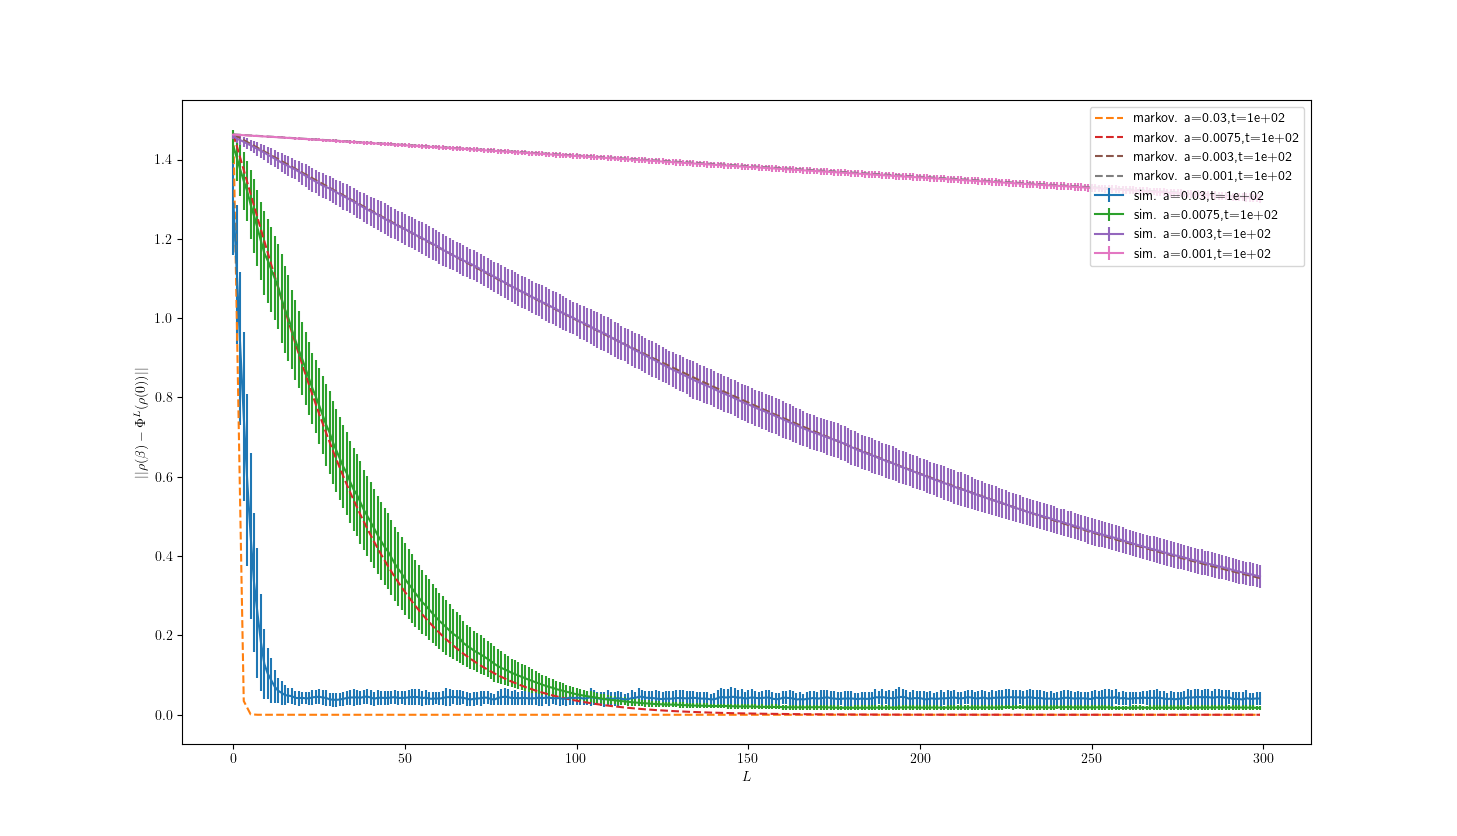
\includegraphics[width=0.45\linewidth]{numerics/data/sho_error_vs_l.png}
    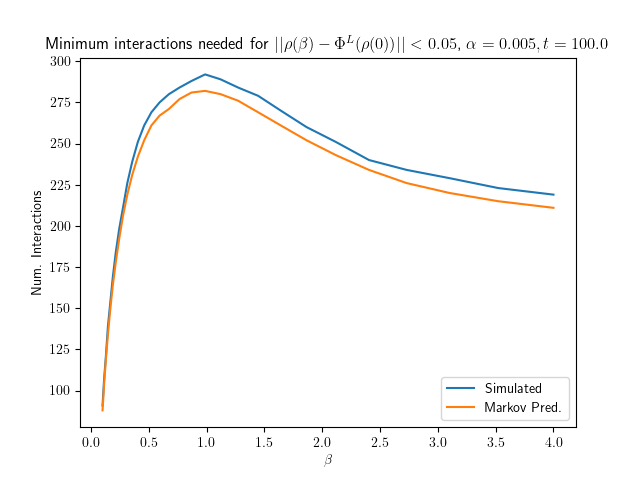
\includegraphics[width=0.45\linewidth]{numerics/data/sho_l_vs_beta.png} \\
    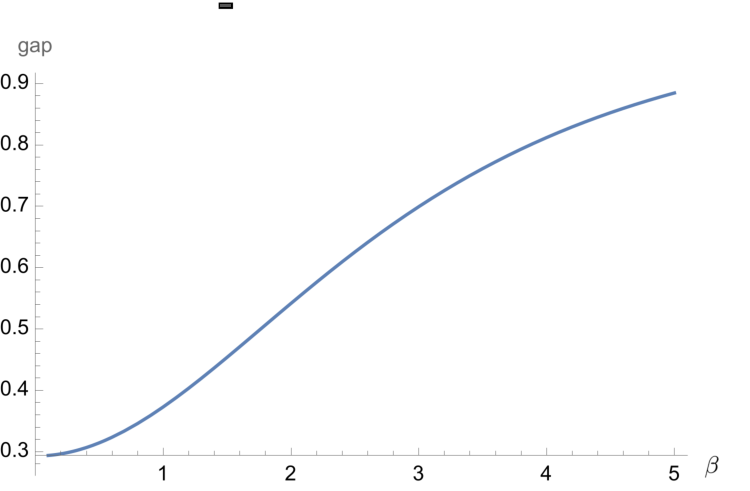
\includegraphics[width=0.5\linewidth]{numerics/data/spec_gap_dim_4.pdf}
    \caption{TODO: Improve. Trace distance to target as a function of interaction number, simulation compared to Markov chain behavior. The Hilbert-Schmidt overlap with the ground state $\anglebrackets{\Phi^L(\rho(0)), \ketbra{0}{0}}$ is 0.940 at $L = 300$. }
    \label{fig:enter-label}
\end{figure}

The behavior of the fixed $\epsilon$ plot reveals a very interesting phenomenon where the number of interactions, and therefore total thermalization time, needed to reach the thermal state goes \emph{down} after a peak at about $\beta = 1.0$. This means colder temperatures can be reached quicker than some intermediate temperatures, assuming a starting state of the maximally mixed state. Our rationale for this behavior is that the spectral gap of the resulting Markov chain must increase with $\beta$ faster than the distance from $\rho(0)$ to $\rho(\beta)$ grows with $\beta$. This bears out when we plot the spectral gap as a function of $\beta$ for the truncated harmonic oscillator, seen in Fig. \ref{fig:enter-label}.

Once we have determined how the thermalization process behaves for a given $\alpha$ and $t$, we can then sweep these parameters to determine how they effect thermalization. From our analysis of the single qubit case we would expect that the distance to the Markov chain can be made arbitrarily close as we both reduce the off-resonant terms by making $\alpha$ smaller and reducing the norm of the remainder terms by making $\widetilde{\alpha}$ smaller. As $t$ is not set we can choose which one to reduce by also varying $t$. As $t$ dictates the simulation time for the system dynamics we would like to reduce it as much as possible. The plot povided in Fig [TODO] shows that the total simulation time 

\begin{figure}
    \centering
    \includegraphics[width=0.5\linewidth]{num}
    \caption{Caption}
    \label{fig:enter-label}
\end{figure}

\section{General Systems}
 Now that we have studied a single qubit and the harmonic oscillator in as much detail as possible, in this section we explore the behavior of our algorithm for some more generic systems. As we have shown the dynamics of the thermalizing channel boils down to a Markov chain over the eigenstates, meaning that without (or even with) special structure it is nearly impossible to provide runtime bounds 

 
For a generic system it becomes very difficult to make any results without promises about our knowledge of the Hamiltonian. Right away the most obvious problem is that without prior knowledge we have no clue really what value of $\gamma$ we should tune our ancilla qubits to. For the single qubit and harmonic oscillator case we had complete knowledge of the spectrum of $H_S$. One thing we would like to show is that it is possible to do so if we also know the spectrum of $H_S$ completely. This will involve randomly choosing a value of $\gamma$ from the Bohr frequency set with importance sampling. Even with these promises it turns out to be incredibly difficult to analyze the resulting Markov chain for an arbitrary $\beta$. What we will do instead of an arbitrary thermal state preparation is to instead prepare the ground state. As an additional preprocessing step one could apply a filter function like a Heaviside step function to the Hamiltonian, thus eliminating the need for knowledge of eigenvalue gaps. This route was analyzed using Quantum Signal Processing (QSP) techniques in (Cite Danial dynamical cooling). 


\subsection{Ground State Preparation}

To see that the ground state is a fixed point, not necessarily the unique fixed point, of the process as $\beta_E \to \infty$ is pretty straightforward; all we have to do is show that the vector $e_1$ is in the nullspace of $T$, or that the first column of $T$ approaches 0. For now we will assume an arbitrary fixed value of $\gamma$. We will first compute the transition amplitudes to the ground state for excited states ($i \neq 1$)
\begin{align}
    \bra{i} \mathcal{T}_{\on}(\ketbra{1}{1} ) \ket{i} &= \widetilde{\alpha}^2 \frac{e^{-\beta \gamma}}{1 + e^{-\beta \gamma}} \sinc^2\left(\frac{(\Delta(i, 1) - \gamma)t}{2} \right),
\end{align}
which we see goes to 0 for any $\gamma$ as $\beta \to \infty$. As $\bra{1}\mathcal{T}_{\on}(\ketbra{1}{1}) \ket{1} = - \sum_{i > 1} \bra{i} \mathcal{T}_{\on}(\ketbra{1}{1} ) \ket{i}$, the self-transition term also approaches 0. Therefore the state $\ketbra{1}{1}$, which in classical land is $e_1$, is a fixed point of the dynamics if the ground state of the environment (a.k.a the computational basis state $\ket{0}$) can be prepared exactly. Standard error propagation arguments should be able to convert the error in state preparation of the environment to showing that the ground state is approximately fixed. 


\subsection{Perfect $\lambda(i) - \lambda(j)$ Knowledge}
Given that our thermalization procedure boils down to a Markov chain that is dependent on tuning our environment gap $\gamma$ to eigenvalue differences $\Delta(i,j)$ we cannot prove much for general systems without some promises. For the Harmonic oscillator we are promised that each eigenstate has a neighboring eigenstate with energy $\pm \Delta$. For a generic system we will work with the promise that 
Now we want to look at systems in which the eigenvalue differences are unique, aka for $i \neq k, \Delta_S(i, j) \neq \Delta_S(k, l)$. in this scenario by taking $t$ to be larger than the smallest eigenvalue difference we can selectively drive transitions among states by tuning $\gamma$ to be equal to their gap. In symbols, we need $t > \min_{(i, j) \neq (k, l)} \left| \Delta_S(i, j) - \Delta_S(k,l)\right| $. This ensures that choosing $\gamma = \Delta_S(i,j)$, for $i < j$ the on-resonance transitions (for off-diagonal elements) will look like:
\begin{equation}
    \bra{l} \mathcal{T}_{\on}(\ketbra{k}{k}) \ket{l} = \widetilde{\alpha}^2 \frac{e^{-\beta \Delta(i,j)}}{1 + e^{-\beta \Delta(i, j)}} \mathbf{I}[(k,l) = (i, j)].
\end{equation}
We use the notation $q(0; i,j) \coloneqq \frac{1}{1 + e^{-\beta \Delta(i,j)}}$ and $q(1;i, j) = 1 - q(0;i,j)$.
The resulting on-resonance matrix will have only two off-diagonal elements and the rest will be off-resonance and therefore negligible. Now by choosing $\gamma$ from these eigenvalue differences uniformly at random, we can build an all-to-all, uniform Markov chain with resulting on-resonance transition matrix:
\begin{align}
    \mathbb{E}_{\gamma} \bra{l} \mathcal{T}_{\on}(\ketbra{k}{k}) \ket{l} = \widetilde{\alpha}^2 \frac{2}{\dim_S(\dim_S - 1)} \left(q(0; k, l) \mathbf{I}[k > l] + q(1; k,l) \mathbf{I}[k < l] \right)
\end{align}
As we can see these transition coefficients are uniform and only change if the state loses or gains energy. The diagonal entries then depend on the number of states with energy greater than the given eigenstate. 
\begin{align}
    \mathbb{E}_{\gamma} \bra{i} \mathcal{T}_{\on}(\ketbra{i}{i}) \ket{i} &= - \frac{2\widetilde{\alpha}^2}{\dim_S(\dim_S - 1)} \left(\sum_{j < i} q(0; i, j) + \sum_{j > i} q(1; i, j) \right)
\end{align}

To show that the thermal state is a fixed point we need to show that it is in the kernel of $T$. This means we can ignore the prefactors, as they are uniform for every matrix element. Computing the first column of $T p_{\beta}$, which is $e_1^T T \vec{p}_{\beta}$ and further we will ignore the constant prefactor of $\frac{2 \widetilde{\alpha}^2}{\dim_S (\dim_S - 1)}$, we get
\begin{align}
    e_1^T T e_1 &= - \sum_{j > 1} q(1; 1, j) = -\sum_{j > 1} \frac{e^{-\beta \Delta(j, 1)}}{ 1 + e^{-\beta \Delta(j, 1)}} \\
    j > 1 \implies e_1^T T e_j &= q(0; j, 1) = \frac{1}{1 + e^{-\beta \Delta(j,1)}}.
\end{align}
The weighted sum with respect to the Boltzmann distribution should therefore be zero if we want it to be a fixed point
\begin{align}
    e_1^T T \vec{p}_{\beta} &= \frac{1}{\partfun(\beta)} \left( -e^{-\beta \lambda(1)} \sum_{j > 1} \frac{e^{-\beta \Delta(j, 1)}}{1 + e^{-\beta \Delta(j,1)}} + \sum_{j>1} e^{-\beta \lambda(j)} \frac{1}{1 + e^{-\beta \Delta(j, 1)}}\right) \\
    &= \frac{1}{\partfun(\beta)} \sum_{j > 1} -\frac{e^{-\beta \lambda(j)}}{1 + e^{-\beta \Delta(j, 1)}} + \frac{e^{-\beta \lambda(j)}}{1 + e^{-\beta \Delta(j, 1)}} \\
    &= 0.
\end{align}
We will compute an arbitrary middle point just for completeness' sake
\begin{align}
    e_j^T T \vec{p}_{\beta} &= \frac{1}{\partfun(\beta)} \left( -e^{-\beta \lambda(j)} \left(\sum_{k < j} q(0;j, k) + \sum_{k > j} q(1;j,k) \right) + \sum_{k < j} e^{-\beta \lambda(k)} q(1; j,k) + \sum_{k > j} e^{-\beta \lambda(k)} q(0; j,k) \right) \\
    &= \frac{1}{\partfun(\beta)} \left( \sum_{k < j} (-e^{-\beta \lambda(j)} q(0; j, k) + e^{-\beta \lambda(k)} q(1; j,k)) + \sum_{k > j} (-e^{-\beta \lambda(j)} q(1;j,k) + e^{-\beta \lambda(k)} q(0;j,k)) \right) \\
    &= \frac{1}{\partfun(\beta)} \left( \sum_{k < j} \left( - \frac{e^{-\beta \lambda(j)}}{1 + e^{-\beta \Delta(j,k)}} + \frac{e^{-\beta (\lambda(k) + \Delta(j, k))}}{1 + e^{-\beta \Delta(j,k)}} \right) + \sum_{k > j} \left(-\frac{e^{-\beta(\lambda(j) + \Delta(k,j ))}}{1 + e^{-\beta \Delta(k,j)}} + \frac{e^{-\beta\lambda(k)}}{1 + e^{-\beta \Delta(k,j)}} \right) \right) \\
    &=0.
\end{align}
 where we remind the reader that we only sample $\gamma$ from positive eigenvalue differences which explains why the $k > j$ sum has $\Delta(k,j) = \lambda(k) - \lambda(j)$. The last row $e_{\dim_S}^T T \vec{p}_{\beta}$ is computed similarly to the first row and is also 0. Conservation of probability arguments can also be made to show that it is zero without computing it. 

One last note is that this Markov chain is clearly ergodic, as the probability for any state to transition to an arbitrary state $j$ from arbitrary starting state $j$ is given by $e_j^T(I + T)e_i$, which is nonzero for all $i, j$ due to our random sampling of the eigenvalue difference $\Delta(i,j)$. Ergodicity tells us that the thermal state is indeed the unique fixed point. 

One could possibly extend this argument for non-unique eigenvalue differences. For example in the Harmonic Oscillator, as studied before, the eigenvalue differences are highly degenerate; this is what allows us to get away with using just a single value of $\gamma = \Delta$ to prepare the thermal state. If we let $\eta(i,j)$ denote the number of eigenvalue differences with value $\Delta(i, j)$ and sample an eigenvalue difference as if we uniformly choose eigenvalue $i$ and then uniformly choose $j \neq i$ (and then take the absolute value) the probability of choosing $\Delta(i,j)$ is $\frac{2 \eta(i,j)}{\dim_S (\dim_S - 1)}$. Then the (off-diagonal) values of $T$ will look like
\begin{equation}
    \mathbb{E}_{\gamma} e_j^T T e_i = \frac{2 \widetilde{\alpha}^2 \eta(i,j)}{\dim_S(\dim_S - 1)} \left( q(0;i,j) \mathbf{I}[i > j] + q(1;i,j) \mathbf{I}[i < j]\right). 
\end{equation}
By tacking on values of $\eta(i,j)$ wherever they need to go we can then compute an arbitrary row of $T \vec{p}_{\beta}$ as
\begin{align}
    \mathbb{E}_{\gamma} e_k T \vec{p}_{\beta} &= \frac{1}{\partfun(\beta)} \left(\sum_{i < k} e^{-\beta \lambda(i)} \mathbb{E}_{\gamma} e_k^T T e_i + e^{-\beta \lambda(k)} \mathbb{E}_{\gamma} e_k^T T e_k + \sum_{i > k} e^{-\beta \lambda(i)} \mathbb{E}_{\gamma} e_k^T T e_i \right) \\
    &= \frac{2 \widetilde{\alpha}^2}{d(d - 1) \partfun(\beta)} \left(\sum_{i < k} \eta(i,k) (e^{-\beta \lambda(i)} q(1; i,k) - e^{-\beta \lambda(k)} q(0; i,k) ) + \sum_{i > k} \eta(i,k)(e^{-\beta \lambda(i)} q(1;i,k) - e^{-\beta \lambda(k)} q(0;i,k))\right) \\
    &= 0,
\end{align}
where the 0 follows the exact same algebra as the unique eigenvalue differences case. 


 \subsection{Hydrogen Chains}
 We report on numeric investigations on the performance of this algorithm for simple Hydrogen chain systems, a common benchmarking system for the performance of quantum chemistry algorithms. We will run a basic implementation of this algorithm, using exact matrix exponentiation to implement the time evolution operators $e^{\pm i (H_S + H_E + \alpha G)t}$ and measure the trace distance to the exact thermal state, also computed using matrix exponentiation. We will use rather conservative choices of $\alpha = 0.001$ and $t = 100.0$ for all hydrogen chains. To choose $\gamma$ we will sample a value randomly from a Gaussian random variable centered at the average eigenvalue of $H_S$, computed using the trace identity $\trace{H_S} = \sum \lambda(i)$ and divide by the dimension of the Hilbert space. 

\bibliographystyle{unsrt}
\bibliography{bib}

\appendix



\section{Sinc Function}

\begin{lemma}[Sinc Function Bounds] \label{lem:sinc_poly_approx}
    The following implications hold 
    \begin{align}
        |x| \leq \sqrt{10 \epsilon_{\sinc}/7} &\implies \sinc^2(x) \geq 1 - \epsilon_{\sinc} \label{eq:sinc_lower_bound}\\
        |x| \geq 1 / \sqrt{\epsilon_{\sinc}} &\implies \sinc^2(x) \leq \epsilon_{\sinc}. \label{eq:sinc_upper_bound}
    \end{align}
    % The constant approximation $f(x) = 1$ has error $|f(x) - 1| \leq \widetilde{\epsilon}_{\sinc}$ if $|x| \leq \sqrt{2 \widetilde{\epsilon}_{\sinc}}$. This leads to the observation that $\widetilde{\epsilon}_{\sinc}$ acts as a lower bound for $f(x)$, as $|x| \leq \sqrt{2 \widetilde{\epsilon}_{\sinc}}$ implies $f(x) \geq 1 - \widetilde{\epsilon}_{\sinc}$. We denote this upper bound with $\Delta_{\sinc} \coloneqq \sqrt{2 \widetilde{\epsilon}_{\sinc}}$. 
    % We also require a lower bound $\epsilon_{\sinc}$, such that $|x| \geq \Delta_{\min} \implies f(x) \leq \epsilon_{\sinc}$. Setting $\Delta_{\min} = 1 / \sqrt{\epsilon_{\sinc}}$ guarantees this to hold. 
\end{lemma}
\begin{proof}
    We start with a Taylor Series for $\sinc^2$, which we compute using the expression of $\sinc$ as $\sinc(x) = \frac{\sin x}{x} = \int_0^1 \cos(sx) ds$. We compute the first two derivatives as
    \begin{align}
        \frac{d \sinc^2(x)}{dx} &= -2 \int_0^1 \sin(sx) s ds \int_0^1 \cos(sx) ds \\
        \frac{d^2 \sinc^2(x)}{dx^2} &= -2 \int_0^1 \cos(sx)s^2 ds \int_0^1 \cos(sx) ds + 2\int_0^1 \sin(sx) s ~ds \int_0^1 \sin(sx) s ~ds.
    \end{align}
    We can evaluate each of these derivatives about the origin using continuity of the derivatives along with the limits $\lim_{x \to 0} \cos(sx) = 1$ and $\lim_{x \to 0} \sin(sx) = 0$. We can now compute the Maclaurin Series for some $x_{\star} \in [0,1]$ as
    \begin{align}
        f(x) &= f(0) + x \frac{df}{dx}\bigg|_{x = 0} + \frac{x^2}{2!} \frac{d^2f}{dx^2}\bigg|_{x = x_{\star}}.
    \end{align}
    Plugging in $\sinc^2(0) = 1$ and $\frac{d\sinc^2(x)}{dx}\big|_{x = 0} = 0$ then yields $|\sinc^2(x) - 1| = \frac{|x|^2}{2} \abs{\frac{d^2\sinc^2(x)}{dx^2}(x_{\star})}$. We make use of the rather simplistic bound
    \begin{align}
        \abs{\frac{d^2\sinc^2(x)}{dx^2}(x_{\star})} &\leq 2 \abs{\int_0^1 \cos(sx) s^2 ds \int_0^1 \cos(sx) ds} + 2\abs{\int_0^1 \sin(sx) s ds \int_0^1 \sin(sx) s ds} \\
        &\leq 2 \int_0^1 \abs{\cos(sx)} s^2 ds \int_0^1 \abs{\cos(sx)} ds + 2\parens{\int_0^1 \abs{\sin(sx)} |s| ds}^2 \\
        &\leq 2 \int_0^1 s^2 ds + 2\parens{\int_0^1 s ds}^2 \\
        &\leq 2/3 + 1/2 = 7/6.
    \end{align}
    This yields the final inequality $|\sinc^2(x) - 1| \leq \frac{7|x|^2}{10}$. We then see that $|x| \leq \sqrt{10 \widetilde{\epsilon}_{\sinc}/7}$ implies $|f(x) - 1| \leq \widetilde{\epsilon}_{\sinc}$. 

    The upper bound of $\epsilon_{\sinc}$ for large $|x|$ is relatively straightforward:
    \begin{align}
        f(x) &= \frac{\sin^2(x)}{x^2} \\
            &\leq \frac{1}{|x|^2},
    \end{align}
    where we see that $|x| \geq 1 / \sqrt{\epsilon_{\sinc}}$ implies $\sinc^2(x) \leq \epsilon_{\sinc}$.
\end{proof}

We will often rely on a particularly parametrized form of $f(x)$ which is worth investigating on it's own right. Note we can get a square root improvement of the dependence of $|\Delta_S(i,j) - \gamma|$ on $\epsilon_{\sinc}$ in the below Corallary if we only require $f(x) \geq 1 - \widetilde{\epsilon}_{\sinc}$. This then requires $|\Delta_S(i,j) - \gamma| \in \bigo{\sqrt{\epsilon_{\sinc} \widetilde{\epsilon}_{\sinc}}}$, however this will not prove significantly useful for us so we use the looser bound.
\begin{corollary} \label{cor:gamma_difference_reqs}
    The statements 
    $$|x| \geq \Delta_{\min} \implies \sinc^2\parens{xt / 2} \leq \epsilon_{\sinc}$$
    and
    $$|x| = |\Delta_S(i,j) - \gamma| \leq \sqrt{2} \Delta_{\min} \epsilon_{\sinc} \implies f(xt/2) \geq 1 - \epsilon_{\sinc}$$
    hold for $t = \frac{2}{\Delta_{\min} \sqrt{\epsilon_{\sinc}}}$. This gives $\epsilon_{\sinc} = \frac{4}{\Delta_{\min}^2 t^2}$. We denote the barrier $\Delta_{\sinc} = \sqrt{2} \Delta_{\min} \epsilon_{\sinc}$. 
\end{corollary}
\begin{proof}
    Throughout this proof we can think of $0 \leq \Delta_{\min} \leq \Delta_S(i,j)$ as a constant, so we avoid writing it as function arguments.
    We first want to provide a bound on $t$ such that $|x| \geq \Delta_{\min}$ implies $f(xt/2) \leq \epsilon_{\sinc}$. This is provided through Eq. \eqref{eq:sinc_upper_bound}
    \begin{align}
        \left| \frac{x t }{ 2} \right| = \frac{|x| t}{2} \geq \frac{\Delta_{\min}t}{2}.
    \end{align}
    We see that setting $t$ such that $\Delta_{\min} t / 2 = 1 /\sqrt{\epsilon_{\sinc}}$, which can be rewritten as $t = \frac{2}{\Delta_{min} \sqrt{\epsilon_{\sinc}}}$, yields the implication $|x| \geq \Delta_{\min} \implies f(xt/2) \leq \epsilon_{\sinc}$. 

    We now want to investigate what values of $x = \Delta_S(i,j) - \gamma$, for the given $t$ as above, yields $f(xt/2) \geq 1 - \epsilon_{\sinc}$. We see that the inequality required for this is
    \begin{align}
        \frac{|x| t}{2} &\leq \sqrt{2 \epsilon_{\sinc}} \\
        \iff  |\Delta_S(i,j) - \gamma| \frac{2}{2 \Delta_{\min} \sqrt{\epsilon_{\sinc}}} &\leq \sqrt{2 \epsilon_{\sinc}} \\
        \iff \abs{\Delta_S(i,j) - \gamma} &\leq \sqrt{2} \Delta_{\min} \epsilon_{\sinc}
    \end{align}
\end{proof}


We now see that if we want there to be unique $(i,j)$ such that $|\Delta_S(i,j) - \gamma| \leq \Delta_{\sinc}$ and for $(i',j') \neq (i,j) \implies |\Delta_S(i',j') - \gamma| \geq \Delta_{\min}$, then we require $|\Delta_S(i,j) - \Delta_S(k,l)| \geq \Delta_{\min} + \Delta_{\sinc}$. 

Suppose $|\Delta_S(i,j) - \gamma| \leq \Delta_{\sinc}$ and $|\Delta_S(i,j) - \Delta_S(k,l)| \geq \Delta_{\sinc} + \Delta_{\min}$ for $(k,l) \neq (i,j)$. We would like to show then that $|\Delta_S(k,l) - \gamma| \geq \Delta_{\min}$. We see that given three real numbers $\gamma, \Delta_S(i,j), \Delta_S(k,l)$ we have four relevant orderings:
\begin{align}
    \gamma \leq \Delta_S(i,j) \leq \Delta_S(k,l) \\
    \Delta_S(k,l) \leq \Delta_S(i,j) \leq \gamma \\
    \Delta_S(i,j) \leq \gamma \leq \Delta_S(k,l) \\
    \Delta_S(k,l) \leq \gamma \leq \Delta_S(i,j).
\end{align}
The scenario $\gamma \leq \Delta_S(i,j) \leq \Delta_S(k,l)$ yields
\begin{align}
    |\Delta_S(k,l) - \gamma| &= \Delta_S(k,l) - \gamma \\
    &= \Delta_S(k,l) - \Delta_S(i,j) + \Delta_S(i,j) - \gamma \\
    &\geq \Delta_S(k,l) - \Delta_S(i,j) \\
    &= |\Delta_S(k,l) - \Delta_S(i,j)| \\
    &\geq \Delta_{\min} + \Delta_{\sinc} \\
    &\geq \Delta_{\min}.
\end{align}
The other direction ($\Delta_S(k,l) \leq \Delta_S(i,j) \leq \gamma$) holds similarly. 

The scenario $\Delta_S(k,l) \leq \gamma \leq \Delta_S(i,j)$ holds through the following computation
\begin{align}
    |\Delta_S(k,l) - \gamma| &= \gamma - \Delta_S(k,l) \\
    &= \gamma + \Delta_S(i,j) - \Delta_S(i,j) - \Delta_S(k,l) \\
    &= \gamma - \Delta_S(i,j) + |\Delta_S(i,j) - \Delta_S(k,l)| \\
    &= -|\gamma - \Delta_S(i,j)| + |\Delta_S(i,j) - \Delta_S(k,l)| \\
    &\geq -\Delta_{\sinc} + \Delta_{\min} + \Delta_{\sinc} \\
    &= \Delta_{\min}.
\end{align}
The other direction ($\Delta_S(i,j) \leq \gamma \leq \Delta_S(k,l)$ ) holds similarly.



\section{Haar Integral Proofs} \label{sec:haar_integral_appendix}

In this section we present the more technical work needed to state our results in Section \ref{sec:taylor_series_phi}. The first two results are Lemmas that compute the effects of the randomized interaction in a form that are usable in the main result of Theorem \ref{lem:big_one}.

\begin{lemma} \label{lem:two_heisenberg_interactions}
    Let $G(t)$ denote the Heisenberg evolved random interaction $G(t) = e^{iHt} G e^{-iHt}$ for a total Hamiltonian $H$. After averaging over the interaction measure the product $G(x) G(y)$ can be computed as
    \begin{equation}
        \int G(x) G(y) dG = \frac{1}{\dim + 1} \parens{\sum_{(i,j),(k,l)} e^{i \Delta(i,j|k,l) (x-y)} \ketbra{i,j}{i,j} + \identity}.
    \end{equation}
\end{lemma}
\begin{proof}
The overall structure of this proof is to evaluate the product in the Hamiltonian eigenbasis and split the product into three factors: a phase contribution from the time evolution, a Haar integral from the eigenvalues of the random interaction, and the eigenvalue contribution of the random interaction. Since this involves the use of multiple indices, it will greatly simplify the proof to use a single index over the total Hilbert space $\hilb$ as opposed to two indices over $\hilb_S \otimes \hilb_E$. For example, the index $a$ should be thought of as a pair $(a_s, a_e)$, and functions $\lambda(a)$ should be thought of as $\lambda(a_s, a_e)$. Once the final form of the expression is reached we will substitute in pairs of indices for easier use of the lemma in other places.
    \begin{align}
        \int G(x) G(y) dG &= \int e^{+i H x} U_G D U_G^\dagger e^{-i H x} e^{+i H y} U_G D U_G^\dagger e^{-i H y} dU_G ~dD \\
        &= \int \bigg[\sum_a e^{+i \lambda(a)x}\ketbra{a}{a}  U_G \sum_b D(b)\ketbra{b}{b} U_G^\dagger \nonumber \\
        &\quad \sum_c e^{-i \lambda(c) (x - y)} \ketbra{c}{c} U_G \sum_d D(d)\ketbra{d}{d} U_G^\dagger \sum_e e^{-i \lambda(e) y} \ketbra{e}{e} \bigg] dU_G ~dD\\
        &=\sum_{a,b,c,d,e} \ketbra{a}{e} e^{-i (\lambda(c) - \lambda(a))x} e^{-i (\lambda(e) - \lambda(c))y} \nonumber \\
        &\quad \times \int \bra{a} U_G \ket{b} \bra{c} U_G \ket{d} \bra{b} U_G^{\dagger} \ket{c} \bra{d} U_G^\dagger \ket{e} dU_G \int D(b) D(d) dD \\
        &=  \sum_{a, b, c, d, e} \delta_{bd} \ketbra{a}{e} e^{-i (\lambda(c) - \lambda(a))x} e^{-i (\lambda(e) - \lambda(c))y} \nonumber \\
        &\quad \times \int \bra{a} U_G \ket{b} \bra{c} U_G \ket{d} \bra{b} U_G^{\dagger} \ket{c} \bra{d} U_G^\dagger \ket{e} dU_G. \\
    \end{align}
    Now the summation over $d$ fixes $d=b$ and we use Lemma \ref{lem:haar_two_moment} to compute the Haar integral, which simplifies greatly due to the repeated $b$ index. Plugging the result into the above yields the following
    \begin{align}
        &= \frac{1}{\dim^2 - 1} \sum_{a, b, c, e} \ketbra{a}{e} e^{-i (\lambda(c) - \lambda(a))x} e^{-i (\lambda(e) - \lambda(c))y} \parens{\delta_{ac} \delta_{ce} + \delta_{ae} - \frac{1}{\dim} \parens{\delta_{ac} \delta_{ce} + \delta_{ae}}}  \\
        &= \frac{1}{\dim^2 - 1} \parens{1 - \frac{1}{\dim}} \sum_{a, b, c, e} \ketbra{a}{e} e^{-i (\lambda(c) - \lambda(a))x} e^{-i (\lambda(e) - \lambda(c))y} \delta_{ae} (1 + \delta_{ac}) \\
        &= \frac{1}{\dim^2 - 1} \parens{1 - \frac{1}{\dim}} \sum_{a, b, c} \ketbra{a}{a} e^{i (\lambda(a) - \lambda(c))(x-y)} (1 + \delta_{ac}) \\
        &= \frac{1 \parens{\dim - 1}}{\dim^2 - 1} \sum_{a,c} \ketbra{a}{a} e^{i (\lambda(a) - \lambda(c))(x - y)} (1 + \delta_{ac}) \\
        &= \frac{1}{\dim + 1} \parens{\sum_{a,c} e^{i (\lambda(a) - \lambda(c))(x-y)} \ketbra{a}{a} + \identity}.
    \end{align}
    Reindexing by $a \mapsto i,j$, $c \mapsto k,l$, and plugging in the definition of $\Delta$ yields the statement of the lemma.
\end{proof}


\begin{lemma} \label{lem:sandwiched_interaction}
    Given two Heisenberg evolved random interactions, $G(x)$ and $G(y)$, we compute their action on an outer-product $\ketbra{i,j}{k,l}$ as
    \begin{equation}
        \int G(x) \ketbra{i,j}{k,l} G(y) ~dG = \frac{1}{\dim + 1} \parens{\ketbra{i,j}{k,l} + \delta(i,j|k,l) \sum_{m,n} e^{i \Delta(m,n | i,j) (x-y)} \ketbra{m,n}{m,n}}
    \end{equation}
\end{lemma}
\begin{proof}
This proof is structured the same as Lemma \ref{lem:two_heisenberg_interactions} and similarly we will use a single index of the total Hilbert space $\hilb$ and switch to two indices to match the rest of the exposition.
    \begin{align}
        \int G(x) \ketbra{a}{b} G(y) dG &=  \int e^{i H x} U_G D U_G^{\dagger} e^{-i H x} \ketbra{a}{b} e^{i H y} U_G D U_G^\dagger e^{-i H y} ~dG \\
        &= \sum_{c, d, e, f} e^{i (\lambda(c) - \lambda(a))x} e^{i (\lambda(b) - \lambda(f))y} \nonumber \\
        &\quad \times \int \ketbra{c}{c} U_G D(d) \ketbra{d}{d} U_G^\dagger \ketbra{a}{b} U_G D(e) \ketbra{e}{e} U_G^\dagger \ketbra{f}{f} dG \\
        &= \sum_{c, d, e, f}  e^{i (\lambda(c) - \lambda(a))x} e^{i (\lambda(b) - \lambda(f))y} \ketbra{c}{f} \nonumber \\
        &\quad \times \int D(d) D(e) dD \int \bra{c} U_G \ket{d} \bra{b} U_G \ket{e} \bra{d} U_G^\dagger \ket{a} \bra{e} U_G^\dagger \ket{f} dU_G \\
        &=  \sum_{c,d,f} e^{i (\lambda(c) - \lambda(a))x} e^{i (\lambda(b) - \lambda(f))y} \ketbra{c}{f} \nonumber \\ 
        &\quad \times \int \bra{c} U_G \ket{d} \bra{b} U_G \ket{d} \bra{a} \overline{U_G} \ket{d} \bra{f} \overline{U_G} \ket{d} dU_G \\
        &= \frac{1}{\dim^2 - 1} \sum_{c,d,f} e^{i (\lambda(c) - \lambda(a))x} e^{i (\lambda(b) - \lambda(f))y} \ketbra{c}{f} (\delta_{ca} \delta_{bf} + \delta_{cf}\delta_{ab})\parens{1 - \frac{1}{\dim}} \\
        &= \frac{1}{\dim + 1} \sum_{c,f} e^{i (\lambda(c) - \lambda(a))x} e^{i (\lambda(b) - \lambda(f))y} \ketbra{c}{f} (\delta_{ca} \delta_{bf} + \delta_{cf}\delta_{ab}) \\
        &= \frac{1}{\dim + 1} \parens{\ketbra{a}{b} + \delta_{ab} \sum_{c} e^{i(\lambda(c) - \lambda(a))(x-y)} \ketbra{c}{c} }.
    \end{align}
    Now re-indexing by $a \mapsto (i,j)$, $b \mapsto (k,l)$ and $c \mapsto (m,n)$ results in the expression given in the statement of the lemma.
\end{proof}


\secondOrderChannelHaar*
\begin{proof}
To start we would like to note that we will use a single index notation to refer to the joint system-environment eigenbasis during this proof to help shorten the already lengthy expressions. We will convert back to a double index notation to match the statement of the theorem. We start from the expression for the first derivative of the channel $\frac{\partial}{\partial \alpha} \Phi_G(\rho_S)$ given by Eq. \eqref{eq:first_order_alpha_derivative}. To take the second derivative there are six factors involving $\alpha$, so we will end up with six terms. We repeat Eq. \eqref{eq:first_order_alpha_derivative} below, add a derivative, and label each factor containing an $\alpha$ for easier computation
\begin{align}
    \frac{\partial^2}{\partial \alpha^2} \Phi_G(\rho_S) =& \frac{\partial}{\partial \alpha} \parens{\int_{0}^{1} \underset{\substack{\downarrow \\ (A)}}{e^{i s (H+\alpha G)t}} (i t G) \underset{\substack{\downarrow \\ (B)}}{e^{i (1-s) (H+\alpha G)t}} ds ~ \rho \underset{\substack{\downarrow \\ (C)}}{e^{-i(H+\alpha G)t}} } \nonumber \\
    &~ ~+\frac{\partial}{\partial \alpha} \parens{ \underset{\substack{\downarrow \\ (D)} }{e^{i(H+\alpha G)t}} \rho \int_{0}^1 \underset{\substack{\downarrow \\ (E)} }{e^{-i s (H+\alpha G) t} } (- i t G) \underset{\substack{\downarrow \\ (F)}}{e^{-i (1-s) (H+\alpha G)t}} ds }.
\end{align}
Our goal is to get each of these terms in a form in which we can use either Lemma \ref{lem:two_heisenberg_interactions} or \ref{lem:sandwiched_interaction}. 
\begin{align}
    (A) &=i t\int_0^1 \parens{\frac{\partial}{\partial \alpha} e^{i s_1 (H+ \alpha G)t}} G e^{i(1-s_1)(H+\alpha G)t} ds_1 \rho e^{-i (H+\alpha G)t} \bigg|_{\alpha=0} \\
    &= (it)^2 \int_0^1 \parens{\int_0^1 e^{i s_1 s_2 (H+\alpha G)t} s_1 G e^{i s_1 (1-s_2) (H+\alpha G)t} ds_2} G e^{i(1-s_1) (H+\alpha G)t} ds_1 \rho e^{-i(H+\alpha G) t} \bigg|_{\alpha=0} \label{eq:second_order_deriv_intermediate_a}\\
    &= -t^2 \int_0^1 \int_0^1 e^{i s_1 s_2 H t} G e^{-i s_1 s_2 H t} e^{i s_1 H t} G e^{-i s_1 H t} s_1 ds_1 ds_2 e^{i H t} \rho e^{-i H t} \\
    &= -t^2 \int_0^1 \int_0^1 G(s_1 s_2 t) G(s_1 t) s_1 ds_1 ds_2 \rho(t). \label{eq:second_deriv_alpha_first_term}
\end{align}

\begin{align}
    (B) &= it \int_0^1 e^{i s_1 (H + \alpha G)t} G \frac{\partial}{\partial \alpha}\parens{e^{i(1-s_1)(H + \alpha G)t}} ds_1 \rho e^{-i(H + \alpha G) t} \bigg|_{\alpha = 0} \\
    &= (it)^2 \int_0^1 e^{i s_1 (H + \alpha G)t} G \parens{\int_0^1 e^{i(1-s_1)s_2 (H + \alpha G)t} (1-s_1) G e^{i(1 - s_1)(1 - s_2)(H + \alpha G)t} ds_2} ds_1 ~ \rho e^{-i ( H + \alpha G)t} \bigg|_{\alpha = 0} \\
    &= -t^2 \int_0^1 \int_0^1 e^{i s_1 H t} G e^{i(1-s_1)s_2 H t} G e^{i(1-s_1)(1-s_2) H t} (1-s_1) ds_1 ds_2 ~ \rho e^{-i H t}\\ 
    &= -t^2 \int_0^1 \int_0^1 e^{i s_1 H t} G e^{-i s_1 H t} e^{i(s_1 + s_2 - s_1 s_2) H t} G e^{-i (s_1 + s_2 - s_1 s_2) H t} (1-s_1) ds_1 ds_2 ~ \rho(t) \\
    &= -t^2 \int_0^1 \int_0^1 G(s_1 t) G((s_1 + s_2 - s_1 s_2)t) (1-s_1) ds_1 ds_2 ~ \rho(t)
\end{align}

\begin{align}
    (C) &= it \int_0^1 e^{i s (H + \alpha G)t} G e^{i(1-s) (H + \alpha G) t} ds ~\rho ~ \frac{\partial}{\partial \alpha} \parens{ e^{-i (H + \alpha G) t} } \bigg|_{\alpha = 0} \\
    &= (i t) (-it) \int_0^1 e^{i s (H + \alpha G)t} G e^{i (1 - s) (H + \alpha G)t} ds ~ \rho ~ \parens{ \int_0^1 e^{-i s (H + \alpha G)t} G e^{-i (1- s) ( H + \alpha G)t } ds}\bigg|_{\alpha = 0} \\
    &= + t^2 \parens{\int_0^1 e^{i s H t} G e^{-i s H t} ds} e^{i H t} \rho e^{-i H t} \parens{\int_0^1 e^{i (1-s) H t} G e^{-i (1-s) H t} ds} \\
    &= + t^2 \int_0^1 G(st) ds ~ \rho(t) \int_0^1 G((1-s)t) ds
\end{align}

\begin{align}
    (D) &= (-it) \frac{\partial}{\partial \alpha} \parens{e^{i(H + \alpha G)t}} \rho \int_0^1 e^{-i s (H + \alpha G)t} G e^{-i (1-s)(H + \alpha G)t} ds \bigg|_{\alpha = 0} \\
    &= t^2 \parens{\int_0^1 e^{i s (H+ \alpha G)t} G e^{i (1-s) (H + \alpha G)t}ds} \rho \int_0^1 e^{-i s (H + \alpha G)t} G e^{-i (1-s)(H + \alpha G)t} ds \bigg|_{\alpha = 0} \\
    &=  t^2 \int_0^1 e^{i s H t} G e^{-i s H t} ds ~\rho(t) \int_0^1 e^{i (1-s) H t} G e^{-i (1-s) H t} ds \\
    &= t^2 \int_0^1 G(st) ds ~ \rho(t) ~ \int_0^1 G((1-s)t) ds
\end{align}

\begin{align}
    (E) &= (-it) e^{i (H+ \alpha G) t} ~ \rho ~\int_0^1 \frac{\partial}{\partial \alpha} \parens{e^{-i s_1 (H + \alpha G)t}} G e^{-i (1-s_1)(H + \alpha G)t} ds_1 \bigg|_{\alpha = 0} \\
    &= - t^2 e^{i(H + \alpha G)t} ~ \rho ~\int_0^1 \parens{\int_0^1 e^{-i s_1 s_2 (H + \alpha G) t} (s_1 G) e^{-i s_1 (1-s_2) (H + \alpha G)t} ds_2} G e^{-i(1-s_1)(H + \alpha G)t} ds_1 \bigg|_{\alpha = 0} \\
    &= -t^2 e^{i H t} \rho e^{-i H t} \int_0^1 \int_0^1 e^{i (1 - s_1 s_2) H t} G e^{-i (s_1 - s_1 s_2)H t} G e^{-i (1-s_1)H t} s_1 ds_1 ds_2 \\
    &= -t^2 \rho(t) \int_0^1 \int_0^1 G((1- s_1 s_2) t) G((1-s_1)t) s_1 ds_1 ds_2
\end{align}

\begin{align}
    (F) &= (-it) e^{i(H + \alpha G) t} \rho \int_0^1 e^{-i s_1 ( H + \alpha G) t} G \frac{\partial}{\partial \alpha} \parens{ e^{-i (1-s_1) ( H +\alpha G)t}} ds_1 \bigg|_{\alpha = 0} \\
    &= (-it)^2 e^{i (H + \alpha G)t} \rho \int_0^1 e^{-i s_1 (H + \alpha G)t} G \parens{\int_0^1 e^{-i(1-s_1) s_2 (H + \alpha G)t} (1-s_1) G e^{-i(1-s_1) (1-s_2) (H + \alpha G) t} ds_2} ds_1 \bigg|_{\alpha = 0} \\
    &= -t^2 e^{-i H t} \rho e^{-i H t} \int_0^1 \int_0^1 e^{i (1- s_1) H t} G e^{-i (1-s_1) H t} e^{i (1-s_1)(1-s_2) H t} G e^{-i(1-s_1)(1-s_2) H t} (1-s_1) ds_1 ds_2 \\
    &= -t^2 \rho(t) \int_0^1 \int_0^1 G((1-s_1)t) G((1-s_1)(1 - s_2) t) (1-s_1)ds_1 ds_2
\end{align}

Now our goal is to compute the effects of averaging over the interaction $G$ on the above terms, starting with $(A)$. As this involves a lot of index manipulations, similarly to the proofs of Lemmas \ref{lem:two_heisenberg_interactions} and \ref{lem:sandwiched_interaction} we will use a single index for the total system-environment Hilbert space and switch back to a double index to state the results. We will make heavy use of Lemma \ref{lem:two_heisenberg_interactions}.
\begin{align}
    \int (A) dG &= -t^2 \int_0^1 \int_0^1 \int G(s_1 s_2 t) G(s_1 t) dG s_1 ds_1 ds_2 \rho(t) \\
    &= \frac{-t^2 }{\dim + 1} \int_0^1 \int_0^1 \parens{\sum_{i,j} e^{i (\lambda(i) - \lambda(j)) (s_1 s_2 t - s_1 t)} \ketbra{i}{i} + \identity} s_1 ds_1 ds_2 \rho(t) \\
    &= \frac{- t^2 }{\dim + 1} \parens{\sum_{i} \sum_{j : \lambda(i) \neq \lambda(j)} \int_0^1 \int_0^1 e^{i(\lambda(i) - \lambda(j))t (s_1 s_2 - s_1)} s_1 ds_1 ds_2 \ketbra{i}{i} + \sum_{i} \sum_{j : \lambda(i) = \lambda(j)}\frac{1}{2} \ketbra{i}{i} + \frac{1}{2} \identity} \rho(t) \\
    &= \frac{- t^2 }{\dim + 1} \parens{\sum_i \sum_{j : \lambda(i) \neq \lambda(j)} \frac{1 - i (\lambda(i) - \lambda(j))t - e^{-i (\lambda(i) - \lambda(j))t}}{t^2 (\lambda(i) - \lambda(j))^2} \ketbra{i}{i} + \frac{1}{2} \sum_{i} (\eta(i) + 1) \ketbra{i}{i} } \rho(t) \\
    &= \frac{- 1}{\dim + 1}\parens{\sum_{i} \sum_{j: \Delta_{ij} \neq 0} \frac{1 - i \Delta_{ij}t - e^{-i \Delta_{ij} t}}{\Delta_{ij}^2} \ketbra{i}{i} + \frac{t^2}{2} \sum_{i} (\eta(i) + 1)\ketbra{i}{i} } \rho(t)
\end{align}

We can similarly compute the averaged $(B)$ term:
\begin{align}
    \int (B) dG &= -t^2 \int_0^1 \int_0^1 \int G(s_1 t) G((s_1 + s_2 - s_1 s_2) t) dG (1-s_1) ds_1 ds_2 ~ \rho(t) \\
    &= \frac{- t^2 }{\dim + 1} \int_0^1 \int_0^1 \parens{\sum_{i,j} e^{i (\lambda(i) - \lambda(j))(s_1 s_2 - s_2) t} \ketbra{i}{i} + \identity} (1 -s_1) ds_1 ds_2 \rho \\
    &= \frac{- t^2 }{\dim + 1} \parens{\sum_{i} \sum_{j : \lambda(i) \neq \lambda(j)} \int_0^1 \int_0^1 e^{i(\lambda(i) - \lambda(j))t (s_1 s_2 - s_2)} (1 - s_1) ds_1 ds_2 \ketbra{i}{i} + \sum_{i} \sum_{j : \lambda(i) = \lambda(j)}\frac{1}{2} \ketbra{i}{i} + \frac{1}{2} \identity} \rho(t) \\
    &= \frac{- t^2 }{\dim + 1} \parens{\sum_i \sum_{j : \lambda(i) \neq \lambda(j)} \frac{1 - i (\lambda(i) - \lambda(j))t - e^{-i (\lambda(i) - \lambda(j))t}}{t^2 (\lambda(i) - \lambda(j))^2} \ketbra{i}{i} + \frac{1}{2} \sum_{i} (\eta(i) + 1) \ketbra{i}{i} } \rho(t) \\
    &= \frac{-1}{\dim + 1}\parens{\sum_{i} \sum_{j: \Delta_{ij} \neq 0} \frac{1 - i \Delta_{ij}t - e^{-i \Delta_{ij} t}}{\Delta_{ij}^2} \ketbra{i}{i} + \frac{t^2}{2} \sum_{i} (\eta(i) + 1)\ketbra{i}{i} } \rho(t),
\end{align}
which we note is identical to $\int (A) dG$. As terms $(C)$ and $(D)$ involve a different method of computation we skip them for now and compute $(E)$ and $(F)$. 
\begin{align}
    \int (E) dG &= -t^2 \rho(t) \int_0^1 \int_0^1 \int G((1- s_1 s_2) t) G((1-s_1)t) dG s_1 ds_1 ds_2 \\
    &= \frac{- t^2}{\dim + 1} \rho(t) \int_0^1 \int_0^1 \parens{\sum_{i,j} e^{i(\lambda(i) - \lambda(j)) t (s_1 - s_1 s_2)} \ketbra{i}{i} + \identity } s_1 ds_1 ds_2 \\
    &= \frac{- t^2}{\dim + 1} \rho(t) \parens{\sum_i \sum_{j : \lambda(i) \neq \lambda(j)} \frac{1 + i (\lambda(i) - \lambda(j))t - e^{i(\lambda(i) - \lambda(j))t}}{t^2 (\lambda(i) - \lambda(j))^2}\ketbra{i}{i} + \frac{1}{2} \sum_{i} (\eta(i) + 1 )\ketbra{i}{i}} \\
    &= \frac{- 1}{\dim + 1} \rho(t) \parens{\sum_i \sum_{j: (\Delta_{ij} \neq 0)} \frac{1 + i \Delta_{ij}t - e^{i\Delta_{ij}t}}{\Delta_{ij}^2} \ketbra{i}{i} + \frac{t^2}{2}\sum_i (\eta(i) + 1) \ketbra{i}{i}}.
\end{align}
Computing $(F)$ yields
\begin{align}
    \int (F) dG &= -t^2 \rho(t) \int_0^1 \int_0^1 \int G((1-s_1)t) G((1-s_1)(1 - s_2) t) dG (1-s_1)ds_1 ds_2 \\
    &= \frac{- t^2 \sigma ^2}{\dim + 1} \rho(t) \int_0^1 \int_0^1 \parens{\sum_{i,j} e^{i(\lambda(i) - \lambda(j))t (s_2 - s_1 s_2)}\ketbra{i}{i} + \identity} (1-s_1) ds_1 ds_2 \\
    &= \frac{- t^2 }{\dim + 1} \rho(t) \parens{\sum_{i} \sum_{j : \lambda(i) \neq \lambda(j)} \frac{1 + i (\lambda(i) - \lambda(j))t - e^{i (\lambda(i) - \lambda(j))t}}{t^2 (\lambda(i) - \lambda(j))^2} \ketbra{i}{i} +\frac{1}{2} \sum_{i} (\eta(i) + 1) \ketbra{i}{i}} \\
    &= \frac{- 1}{\dim + 1} \rho(t) \parens{\sum_i \sum_{j: (\Delta_{ij} \neq 0)} \frac{1 + i \Delta_{ij}t - e^{i\Delta_{ij}t}}{\Delta_{ij}^2} \ketbra{i}{i} + \frac{t^2}{2}\sum_i (\eta(i) + 1) \ketbra{i}{i}}
\end{align}
 which is identical to $\int (E) dG$.

 The last two terms $(C) = (D)$ are computed as follows:
 \begin{align}
     \int (C) dG &= t^2 \int_0^1 \int_0^1 \int G(s_1 t) \rho(t) G((1-s_2)t) ~dG ~ ds_1 ds_2 \\
     &= t^2 \sum_{i,j} \rho_{ij} e^{i(\lambda(i) - \lambda(j))t} \int_0^1 \int_0^1 \int G(s_1 t) \ketbra{i}{j} G((1-s_2)t) ~ dG ~ ds_1 ds_2 \\
     &= \frac{ t^2}{\dim + 1} \sum_{i,j} \rho_{ij} e^{i(\lambda(i) - \lambda(j))t} \parens{ \ketbra{i}{j} + \delta_{ij} \sum_{a} \int_0^1 \int_0^1 e^{i(\lambda(a) - \lambda(i))(s_1 + s_2 - 1)t} ds_1 ds_2 \ketbra{a}{a}} \\
     &= \frac{ t^2}{\dim + 1} \sum_{i,j} \rho_{ij} e^{i \Delta_{ij} t} \parens{\ketbra{i}{j} + \delta_{ij} \sum_{a : \Delta_{ai} \neq 0} \frac{2( 1- \cos (\Delta_{ai} t))}{\Delta_{ai}^2 t^2} \ketbra{a}{a} + \delta_{ij} \sum_{a : \Delta_{ai} = 0} \ketbra{a}{a}}
 \end{align}

 We can now combine each of these terms to offer the full picture of the output of the channel to second order. We make two modifications to the results from each sum: first, we will switch to double index notation to make for easier use in other areas, and secondly we let $\rho = \ketbra{i,j}{k,l}$. We note that the first term in the following equation is provided by $(A) + (B)$, the second through $(E) + (F)$, and the last two through $(C) + (D)$. 
 \begin{align}
     &\int \frac{\partial^2}{\partial \alpha^2} \Phi_G(\ketbra{i,j}{k,l})\bigg|_{\alpha = 0} dG \\
     &= -\frac{2  e^{i \Delta(i,j|k,l) t}}{\dim + 1} \bigg(\sum_{(a,b): \Delta(i,j|a,b) \neq 0} \frac{1 - i \Delta(i,j|a,b)t - e^{-i \Delta(i,j|a,b) t}}{\Delta(i,j|a,b)^2} \nonumber \\
     &~+ \sum_{(a,b): \Delta(k,l|a,b) \neq 0} \frac{1 + i \Delta(k,l|a,b) t - e^{i \Delta(k,l|a,b) t}}{\Delta(k,l|a,b)^2} + \frac{t^2}{2}(\eta(i,j) + \eta(k,l)) \bigg) \ketbra{i,j}{k,l} \nonumber \\
    &~ +\delta_{i,k} \delta_{j,l} \frac{2 e^{i \Delta(i,j|k,l)t}}{\dim+1} \parens{ \sum_{(a,b): \Delta(i,j|a,b) \neq 0 } \frac{2(1- \cos (\Delta(i,j|a,b)t))}{\Delta(i,j|a,b)^2} \ketbra{a,b}{a,b} + t^2 \sum_{(a,b) : \Delta(i,j|a,b) = 0} \ketbra{a,b}{a,b}} \label{eq:second_order_output}
 \end{align}
The last step we need is a quick trig identity (half angle formula) to change the cosine to a sine
\begin{align}
    \frac{2(1 - \cos(\Delta(i,j| a,b)t)}{\Delta(i,j|a,b)^2} &= \frac{2\left( 1 - \left(1 - 2 \sin^2\left(\frac{\Delta(i,j|a,b)t}{2} \right) \right) \right)}{\Delta(i,j|a,b)^2} \\
    &= t^2 \frac{\sin^2 \left(\frac{\Delta(i,j|a,b) t}{2} \right)}{\frac{\Delta(i,j|a,b)^2 t^2}{4}} \\
    &= t^2 \sinc^2 \left(\frac{\Delta(i,j|a,b) t}{2 } \right),
\end{align}
which yields the statement.
\end{proof}





\end{document}